\maketitlepage
%\thispagestyle{fancy}
\section{Introduction}

The Swarm Protocol is a peer-to-peer data storage protocol with a cryptocurrency-based incentive system \cite{book-of-swarm}.
%
Its main deployment, the Swarm Network, currently has over 10,000 active nodes, of which over 5,000 participate in the incentive system\footnote{Conservative estimate based on monthly figures from \cite{soft}.}, collectively earning over USD 25,000 per month\footnote{Based on September figures and token price of USD 0.25.} for storing replicated data in the range of 16--32 tebibytes.\footnote{Based on a replication neighbourhood address space bit depth of $11$, corresponding to 2048 neighbourhoods of 8--16 gibibytes each, as reported at time of writing on \url{https://swarmscan.io/neighborhoods}.}

Customers of the Swarm Network purchase storage quotas in the form of \emph{postage stamp batches} \cite[\S3.3]{book-of-swarm} from a smart contract deployment on Gnosis Chain using the network's native token, the BZZ token.\footnote{\url{https://medium.com/ethereum-swarm/swarm-tokenomics-91254cd5adf}}
%
This revenue is then redistributed among the network's active storage nodes according to a stateful revenue sharing mechanism \cite[\S3.4]{book-of-swarm}.
%
Together with an on-chain price oracle that responds to the apparent replication rate \cite[\S3.4.5]{book-of-swarm}, these supply side control mechanisms have the aim:
%
\begin{quote}
%
  [...] to make it profitable for a node to react in a way that is beneficial for the desired emergent behaviour of the network, while making it costly to act in a way that is detrimental. \hfill\cite[79]{book-of-swarm}
%
\end{quote}


\subsection{Background: scope and objectives}

The object of study in this analysis is the Swarm Protocol revenue sharing mechanism. 
%
We aim to define quantitative economic objectives, evaluate mechanism design choices against these objectives, and suggest avenues for optimisation or further research.

We are particularly interested in the effects of design choices that raise concerns of of node operator incentives being decoupled from service quality or cost, trade barriers that may `freeze' inefficient allocations in place, and NO risk profiles that render small and medium node operations (SMNOs) infeasible.

\subsubsection{Motivation: pitfalls of the revenue sharing mechanism}
\label{section:pitfalls}
%
Due to difficulties in measuring the amount of storage provided by nodes --- particularly in reliably lower bounding the number of replicas being stored --- revenue share allocations in the Swarm Protocol are not based directly on the amount of storage provided.
%
Instead, shares are tracked by an internal `staking' mechanism into which active storage providers must buy \cite[\S3.4.3]{book-of-swarm}.
%
This decoupling raises the question of whether competition for revenue share actually incentivises node operators to improve quality or reduce costs of the service they provide, as might be expected in a more traditional competitive market structure.

Another pitfall arises from the lottery-like nature of payouts --- a feature of many blockchain-based incentive mechanisms --- which imposes disproportionate risk of long periods of zero revenue on small scale node operators \cite{albrecher2022blockchain}.
%
This well-known issue has famously led to the formation of revenue sharing pools in more mature ecosystems with analogous payout structures \cite{rosenfeld2011analysis}.
%
We seek to understand risk measures that could help the Swarm Protocol designers to forecast at what scales this effect will really begin to eat at SMNOs.

\subsubsection{Goals}

The goals of our analysis were as follows:
%
\begin{enumerate}
  \item 
    Establish a set of quantitative objectives for the Swarm revenue share allocation system.

  \item 
    Evaluate to what extent the current design of the revenue sharing mechanism facilitates or impedes these objectives.

  \item 
    Where relevant, propose alternative approaches or avenues of investigation that could lead to improvements on the status quo.
\end{enumerate}
%
Intermediate and side objectives were among the following:
%
\begin{enumerate}[resume]
  \item 
    Describe plausible strategies in the revenue share acquisition game. Try to discover undesirable equilibria.
  
  \item 
    Establish a market clearing model that includes a `quality' parameter tracking replication rate.
  
  \item 
    Describe and evaluate alternative revenue sharing models.

\end{enumerate}

\subsubsection{Methodology}
%
Our approach was to produce a mathematical model of a Swarm Protocol economy that incorporates the details of the revenue sharing mechanism.
%
We then evaluated our model against a list of general economic objectives of the system, understood as a generic service with a single quality parameter.\footnote{The objective functions discussed in the present report are quite different from the list initially reported in August and discussed with V.~Tr\'{o}n.
%
This change occurred because we discovered a way to derive the earlier objectives as intermediate targets from more fundamental economic goals like growth and quality of service.}

In detail, the logical progression of our approach goes as follows:
\begin{enumerate}

  \item 
    Couch the Swarm Protocol economy and its objectives in terms of a general microeconomic production model with objectives of demand, price, and quality, with the latter interpreted as replication rate.
    %
    As protocol designers, we would like to at least achieve a production vector on the efficient frontier of the production set.
  
  \item
    Introduce the notion of an abstract revenue sharing mechanism as a way to construct the feasible production set.
    %
    Efficiency of the resulting production vector then becomes a checkable condition on the revenue sharing mechanism.

  \item
    Exhibit an efficient revenue sharing mechanism under idealised conditions.

  \item
    Describe the Swarm redistribution mechanism as part of a parametrised family (\S\ref{section:model}).

  \item
    Describe the agent policy optimisation problem and establish classes of plausible policies (\S\ref{section:optimal}, \S\ref{section:risk}).
    %
    Observe which allocations (and reallocations) can result, paying particular attention to inefficient outcomes.
    
  \item
    Discuss approaches to estimating or forecasting the unknown or random parameters in the model (\S\ref{section:estimation}).

\end{enumerate}




\subsection{Background: Swarm Protocol overview}
\label{section:overview}

The Swarm Protocol is a decentralised storage service with blockchain-based payments and revenue sharing mechanism.
%
It comprises the following components:
%
\begin{enumerate}
  \item 
    A peer-to-peer network of \emph{storage provider} nodes, each associated with a 256-bit overlay address $a\in\Overlay$;
  \item 
    A utility token deployed on an EVM chain. For the Swarm Network, this is the BZZ token, issued on Etheruem mainnet;
  \item 
    A system of 4 smart contracts that sell storage space on the (nodes participating in the) peer to peer network and redistribute the proceeds among the registered nodes.
    %
    For the Swarm Network, these contracts are deployed on Gnosis Chain, and the unit of account is the xBZZ token, that is, Ethereum mainnet BZZ bridged to Gnosis Chain via the Omnibridge.\footnote{\url{https://docs.gnosischain.com/bridges/About Token Bridges/omnibridge}} 
    %
    (Many sources refer to xBZZ tokens simply as BZZ.)

\end{enumerate}
%
Two types of agents interact with the Swarm Protocol: users, a.k.a.~storage clients, who purchase storage quotas and upload and download data; and node operators (NOs), a.k.a.~storage providers, who provide their storage space and compute storage proofs in exchange for a share of the revenue.
%
The Swarm Network itself can be considered as intermediating between storage clients and storage providers.
%
For more details, see \cite{book-of-swarm}.

\subsubsection{Revenue sharing mechanism}

The topic of study of this report is the Swarm Protocol revenue sharing mechanism design and its effect on the overall system design objectives.
%
\begin{enumerate}
  \item 
    The redistribution mechanism is governed by the Stake Registry and Redistribution contracts.
  
  \item
    The Stake Registry maintains a table of xBZZ-denominated \emph{stake} or \emph{equity balances} associated to each overlay address.\footnote{    Prior to SWIP-19 \cite{swip-19}, share balances were associated to an overlay address.
    %
    Post SWIP-19, balances are associated to a Gnosis chain address together with a derived overlay address \cite{swip-19}.
    %
    That is, after these changes, each Gnosis chain address is associated to a unique share balance, instead of possibly several keyed by different overlay addresses derived using different nonces.}
    %
    These balances are used to control revenue redistribution.

  \item
    Time is divided into \emph{rounds} of 152 Gnosis chain blocks --- targeting 12 minutes 40 seconds.
    %
    The round is further divided into \emph{commit}, \emph{reveal}, and \emph{claim} phases, in that order, with the first two each lasting 38 blocks --- a quarter of a round --- and the third lasting the remaining 76 blocks of the round.

  \item
    Each round, certain selected nodes may submit cryptographic storage proofs to the Redistribution contract for a chance to receive that round's redistributed revenue pot.
    %
    The protocol consists of a commit-reveal scheme followed by a winner selection and payout, with each of the three actions falling into the correspondingly named round.

  \item
    During the Commit phase of the redistribution mechanism, a participating node must commit to a ``depth'' parameter $d$ and the contents of a storage space of non-evictable data called the \emph{reserve}.
    %
    The depth $d$ and the node's overlay address $a\in\Overlay$ together determine a neighbourhood $\Overlay(a,d)\subseteq\Overlay$ of $a$ in address space, comprising the addresses with the same $d$-bit prefix.
    %
    This neighbourhood is the node's claimed \emph{area of responsibility}; it expects all nodes with addresses in $\Overlay(a,d)$ to store the same set of chunks, also with addresses in $\Overlay(a,d)$, as it does.
    
    We also refer to this address space as the \emph{replication bin} claimed by $a$, because it comprises data that ought to be fully replicated among nodes having addresses in $\Overlay(a,d)$.
    %
    That is, the apparent replication rate of data in this range is the number of participating nodes in $\Overlay(a,d)$.

    
  \item
    At commit time, a few additional validity conditions are verified for each participating NO.
    %
    The main ones are:
    \begin{enumerate}
      \item Their equity balance has not been updated within the past 2 rounds.
      \item 
        They are not \emph{frozen} as a penalty for revealing a different hash or depth from the consensus leader or missing a reveal. 
        %
        Freezing penalties last for about 1 day.
      \item 
        They have shares in excess of a minimum threshold $\tau$. For the versions under consideration in this study, $\tau=10$ xBZZ.
    \end{enumerate}

  \item
    During the Reveal phase, NOs reveal the depth and reserve commitment associated to their Commit, and it is checked that the $d$-bit index of the owner node's claimed area of responsibility agrees with the first $d$ bits of a randomness beacon, sampled once each round.\footnote{\url{https://github.com/ethersphere/storage-incentives/blob/v0.8.6/src/Redistribution.sol\#L380}}
    %
    In this way, the active $d$-bit neigbourhood is selected by $d$ bits of randomness.

  \item    
    During the Claim phase, a winner is selected from among those nodes with a valid reveal and which are in agreement with a randomly selected leader.
    %
    Both the consensus leader and winner are selected weighted according to their \emph{stake density}, which in the case that all nodes agree on the value of $d$, is equivalent to weighting by stake/equity balance.
    %
    The winner's storage proofs are then validated, and if valid, the reward is paid out.

  \item
    In this work, we assume that all participating nodes take their depth parameter from a commonly known constant $D$, so in particular they always remain in consensus on the partition of $\Overlay$ into replication bins.
    %
    Moreover, nodes always reveal their commits, agree with the consensus leader on the contents of the reserve, and produce valid proofs.
    %
    They are never frozen.

    At time of writing, $D=11$.



  \item 
    The redistributed revenue is calculated by multiplying the price, as reported by the Price Oracle contract, by the amount of storage consumed, as reported by the Postage contract, at each epoch.
    %
    The computation occurs during the winner selection part of the protocol, triggered by a successful call to \code{claim()}.
    %
    Revenue is denominated in xBZZ tokens.
    %
    The details of this computation are largely out of scope for our model.
  
  \item 
    NOs may increase their equity balance by calling the \code{stakeUpdate()} function of the Stake Registry, paying for equity in xBZZ tokens.
    %
    In the Book of Swarm and related literature, this operation is called \emph{creating} or \emph{topping up stake} \cite[\S3.4.3]{book-of-swarm}.
    
    In this report, we prefer the term \emph{minting shares} as we believe this gives a more accurate mental model of the payoffs and optionality associated with entering into this position.
    %
    This nomenclature also makes it easier to discuss \emph{share prices}, which arise in the consideration of tokenised stake positions in \S\ref{section:tokenisation} and also form a useful mental model for the storage price controlled `committed stake' positions introduced in SWIP-20 \cite{swip-20}.
    %
    That said, we model the version of storage incentives under investigation in this study by setting the share price to a constant $1$.

    In the versions of the Swarm Protocol under study in this analysis, calling \code{stakeUpdate()} is the only way to mutate equity balances.

\end{enumerate}

\subsubsection{Versions}
\label{section:versions}

Our study is based on version 0.8.6 of the storage incentives contracts.\footnote{\url{https://github.com/ethersphere/storage-incentives/tree/v0.8.6}}
%
Since this version only introduced an update to the redistribution contract that is out of scope of the model, our model applies equally well to the versions of contracts deployed at version 0.6.0, or version 0.4.0 in the case of the stake registry.



%%%%%%%%%%%%%%%%%%%%%%%%%%%%%%%%%%%%%%%%%%%%%%%%%%%%%%%%%%%%%%%%%%%%%%%%%%%%%%

\subsection{Findings}

We motivate our findings in terms of the microeconomic objectives of realised demand, redistributed revenue, and apparent replication rate, with the latter understood as a proxy for quality of service.
%
If demand curves are downward sloping, then, maximising demand at a fixed replication rate $q$ is equivalent to achieving the minimal price $p^*(q)$ that the supply side can support.

The Swarm Protocol revenue sharing system governs how the productive capacity of the Swarm Network storage service as a whole emerges from the capacities of individual NOs (\S\ref{section:supply}).
%
Intuitively, we might hope that lower operating costs among the population of potential NOs ought to permit lower prices.
%
However, whether lower operating costs among potential NOs can actually manifest as a lower aggregate cost of providing the Swarm service depends on which NOs decide to add their productive capacity to the storage pool, and hence in turn on the particular manner in which revenue share is allocated among these NOs (\S\ref{section:redistribution}).

If revenue shares are distributed in a \emph{Pareto efficient} manner (Definition \ref{def:efficient}), then the costs, quality, and quantity of the Swarm Network service production vector cannot all be simultaneously improved by some reallocation of shares to more productive NOs.
%
In this case, we can say that the Network \emph{implements} the efficient production vector $(p^*(q),q)$.
%
However, it is not automatic that revenue shares will end up in an efficient allocation.

Our first finding is a positive result on finding efficient revenue share allocations:
%
\begin{theorem}[Corollary \ref{thm:efficient-reallocation-is-possible}]
  
  If stake positions are tokenised and freely tradable with no transaction costs, then from any starting allocation there is a sequence of incentive-compatible trades resulting in a Pareto optimal outcome.

\end{theorem}

However, under the present version of the Swarm Protocol, stake positions are not tokenised and cannot be easily traded or liquidated.
%
We found that under present conditions, the Swarm Protocol revenue sharing system can reach an oligopolistic or monopolistic state where incumbent players can block off market entry opportunities for potential NOs, even if the latter would have lower costs.
%
More productive NOs therefore do not necessarily exert competitive pressure on incumbents to invest in lowering the costs of their own operations.

To formulate this result, we associate to a would-be NO $a$ a measure $c\in(0,1)$ of \emph{cost per unit (network) revenue} (C/R), that is, the ratio of $a$'s operating cost to the redistributed revenue for the whole network.
%
We find that as long as C/R are bounded below uniformaly across all NOs, it's possible for a first mover to monopolise and block entry to a neighbourhood.

\begin{theorem}[Entry blocking]
  \label{thm:block-entry}

  Suppose that the C/R of all NOs are bounded below by a constant $K>0$.
  %
  Let $a$ be an NO with C/R $c$. 
  %
  Suppose that $a$ has an exclusive first-move opportunity to acquire shares in an as-yet unoccupied neighbourhood.
  
  Then for all sufficiently small $c$, there exists a stake position $s$ that $a$ may acquire such that:
  %
  \begin{enumerate}
    \item there is a time-invariant Nash equilibrium in which no new stake updates are made and $a$ remains the sole stakeholder;
    \item it is individually rational for $a$ to make the initial investment $s$; i.e.~$a$ earns at least $s$ in total discounted future profit from his investment at equilibrium.
  \end{enumerate}
  %
  Moreover, $c < \min\{0.32, 2\sqrt{K}-K\}$ is sufficiently small.

\end{theorem}
%
\begin{proof}

  By Proposition \ref{thm:entry-blocking-ratio}, the bound $c<2\sqrt{K}-K$ means that no rational adversary has an entry, assuming $a$ continues operating after the entry.
  %
  On the other hand, by Proposition \ref{thm:no-squeeze}, $c<0.32$ implies that neither will a rational adversary try to `squeeze' $a$ out by diluting him until his costs exceed his income, thereby forcing him to shut down.
  %
  Therefore the only rational move for the adversary is not to play. \qedhere

\end{proof}

Phrased in terms of production vectors, the outlook is negative:

\begin{corollary}

  Under the conditions of Theorem \ref{thm:block-entry}, the Swarm Protocol redistribution mechanism does not implement $(p^*(q),q)$ for any $q>1$.

\end{corollary}


Our third finding is numerical in nature.
%
According to our calculations (Example \ref{smno-calculations}), due to the lottery structure of the reward payout system and based on crude estimates of current environmental parameters, small node operations (of at most 16 nodes) will become unviable due to risk considerations \emph{quite soon}, assuming the network continues to grow at the present rate.
%
Stop-gap measures such as increasing the reserve size (SWIP-21) can delay the effect of this centralisation vector for a few more orders of magnitude of the Network storage capacity, but will eventually run into fundamental barriers when the reserve size needed to make single node operations viable exceeds the capacity of consumer hardware.
%
See \S\ref{section:ruin}.



\subsubsection{Recommendations}
\label{section:recommendations}

\begin{enumerate}
  \item
    We have found theoretical aggressive share minting strategies that lead to illiquid stake allocations that are problematic from an efficiency perspective.
    %
    Empirically, no one is currently pursuing such strategies, but the situation should be carefully monitored.

  \item
    The lack of options to reallocate stake is a potential barrier to economic efficiency and hence optimal pricing.
    %
    The Swarm Protocol designers should consider introducing more reallocation opportunities so that they have an opportunity to undergo real price discovery.
    %
    However, care should be taken to ensure that revenue share does not flow too readily to the the agent with lowest costs, giving it market power.
    
  \item
    As the network grows into the petabyte range, small NO operations such as a single laptop become unviable because of risk of ruin.
    % 
    If demand for Swarm revenue share remains robust, the emergence of stake pools or liquid stake solutions is inevitable.

    The Swarm community should consider what staking pools might look like and whether the core protocol should be changed to either directly support stake pools or facilitate community-led initiatives.


  \item
    The Swarm community should consider how it wishes to prioritise the tradeoff between replication rate (and other QoS) targets and growth targets (realised demand and revenue).
    %
    The particular priority weighting can be expressed in a multi-objective optimisation framework.

\end{enumerate}

\subsubsection{Self-evaluation: did our analysis achieve its goals?}

\begin{enumerate}
  \item 
    \emph{Establish objectives}. 
    %
    We identified fundamental economic objectives of revenue, realised demand, and replication rate, understood as a proxy for quality of service. 
    %
    See \S\ref{section:objectives}.

  \item 
    \emph{Evaluate current design}. 
    %
    Tradeoffs among the three Swarm Network objective functions define a \emph{Pareto efficient frontier}.
    %
    The position of the frontier is determined by the basic economic signals of utility (demand) and cost (supply) of the service.
    
    The revenue sharing system governs how costs of individual operators are aggregated as the cost for the Swarm Network as a whole to provide the storage service at the target replication rate.
    %
    As such, it can affect whether the Swarm Network economic outcome actually lies on the efficient frontier, where Swarm Network service costs reflect the optimal cost-quality tradeoffs available among its node operator population, or not.

  \item 
    \emph{Make recommendations.} 
    %
    The present analysis suggests several concrete directions to explore for addressing the predicted inefficiencies of the Swarm Protocol in its present form.
    %
    However, more thorough work is needed before precise improvement proposals can be made.
    %
    See \S\ref{section:recommendations}.

  \item 
    \emph{Describe strategies and equilibria.} 
    %
    We described several simple strategies and exhibited examples of inefficient equilibria in \S\ref{section:analysis}.
    
    The closed form analytical methods we used are likely insufficient for identifying optimal strategies under more general initial conditions or predicting or ruling out other types of equilibria.
    %
    We expect that approaches based on numerical optimisation methods and computer agent simulation will yield a more complete overview of the strategy profile landscape.
  
  \item 
    \emph{Market clearing model.} See \S\ref{section:efficiency}.
    
  \item 
    \emph{Alternative revenue sharing models.} 
    %
    In \S\ref{section:extensions} we considered variations on the present model introduced by SWIPs that went into production in recent months.
    %
    We also discussed an idealised model of liquid stake positions in \S\ref{section:tokenisation}.

\end{enumerate}




\newpage
%%%%%%%%%%%%%%%%%%%%%%%%%%%%%%%%%%%%%%%%%%%%%%%%%%%%%%%%%%%%%%%%%%%%%%%%%%%%%%%

\section{Objectives of the system design}
\label{section:objectives}

The fundamental goal of the Swarm Protocol incentive system is to entice NOs to provide a storage service that meets potential demand at the desired quality of service (QoS) threshold.
%
The quality target most explicitly encoded into the incentive system is the \emph{replication rate} \cite[\S3.4.5]{book-of-swarm}, which in today's Swarm Network has a target value of $4$,\footnote{\url{https://github.com/ethersphere/storage-incentives/blob/v0.8.6/src/PriceOracle.sol\#L18}} though there are other relevant quality metrics (cf.~Remark \ref{quality-metrics}).

This directly entails three directly measurable dimensions of objectives: realised demand, protocol revenue, and quality in the form of replication rate.

We introduce in \S\ref{section:efficiency} a simple microeconomic model of feasible allocations that includes a `quality' parameter, tracking replication rate, from which we can define an efficient frontier and make basic observations about its geometry.
%
Then, in \S\ref{section:redistribution} we study the core problem of how the choice of redistribution mechanism governs the aggregation of the production capacity of individual nodes into that of the Swarm Network as a whole.
%
With this in mind, it makes sense to ask if a given redistribution mechanism implements an efficient production vector, that is, on the boundary of the set of outputs that could be achieved with an production-optimising redistribution.

In \S\ref{section:decentralisation}


Finally, in \S\ref{section:decentralization} we consider measurement of decentralisation on various axes and its relation to monopoly control of allocation, particularly censorship, and pricing.

\subsection{Objective functions}

We identify three objective functions that exhibit the economic performance of the Swarm network:
%
\begin{enumerate}

  \item Protocol revenue, i.e.~the total cash flows into the Postage contract;

  \item Realised demand, i.e.~the total amount of storage quotas purchased from the Postage contract;

  \item Apparent replication rate, i.e.~the (mean) number of distinct nodes producing successful proofs in the redistribution game each round.\footnote{As discussed above, the true replication rate could be lower than the apparent replication rate because of deduplication/compression.}

\end{enumerate}
%
The target of the revenue and demand objectives is straightforward: the higher the better.
%
We argue that the same is true of the quality objective.


\subsubsection{Realised demand}

The most self-evident success metric of a storage service is the amount of storage purchased.
%
In the Swarm Protocol, realised demand is straightforward to measure as the total size of storage quotas purchased from the Postage contract.

Under the demand theory of ordinary goods, quantity demanded decreases with price, given fixed quality.
%
The demand objective can therefore be transformed into an objective of \emph{price minimisation}, ceteris paribus.
%
See \S\ref{section:demand}.


\subsubsection{Protocol revenue}

If the Swarm Network were a shareholder firm, we might consider \emph{profit maximisation} as a typical objective.
%
The Swarm Network isn't a firm, though, and doesn't have profits in the usual sense.
%
In the current model, all revenue is either redistributed to NOs or, in the case of quotas not fully consumed before expiry, simply locked and effectively removed from circulation.

We propose instead \emph{revenue} as a proxy for the profit maximisation objective because it is straightforward to measure in terms of on-chain flows in and out of the Postage contract.
%
There are two ways to reckon revenue in the Swarm Protocol:
\begin{enumerate}
  \item 
    \emph{Network revenue}, that is, the total BZZ inflows to the Postage contract. 
    %
    Considered marginally, network revenue equals realised demand times price.

  \item 
    \emph{Redistributed revenue}, which is the amount of money \emph{paid out} from the Postage contract via the redistribution mechanism.
    %
    The Swarm Foundation Blog tracks and advertises redistributed revenue in its monthly State of the Network updates.\footnote{\url{https://blog.ethswarm.org/foundation/2024/state-of-the-network-november-2024/\#network-total-monthly-rewards}}

\end{enumerate}
%
In the sequel, we focus on the Network revenue because of its simple relationship to realised demand and storage price.

\begin{remark}[Burn rate]

  It is not uncommon to consider \emph{burn rate} as an objective function in blockchain economies that issue their own token, as is the case for the Swarm Network.
  %
  In the Swarm Protocol today, burn rate is the difference between network revenue and redistributed revenue.
  %
  We don't regard it as an ideal objective for the Swarm storage service because under the current system, it would entail an objective of wasteful spending and non-usage of the service.
  
  Note that payments into the Stake Registry, though not withdrawable in the versions of the contract under analysis here, must not be considered as `burnt' because there exists a mechanism for these tokens to become withdrawable under a protocol upgrade (as in fact has happened under certain conditions downstream of SWIP-20,\footnote{\url{https://github.com/ethersphere/SWIPs/blob/master/SWIPs/swip-20.md}} introduced in the v0.9.1 upgrades).

\end{remark}

\subsubsection{Quality of service}

The stated goal of the Swarm Protocol design is to target a replication rate of 4.
%
We argue that a replication rate of higher than 4 would not be objectionable if it did not negatively impact the other two objectives.
%
Thus replication rate is also a function that we wish to maximise as part of a multi-objective optimisation framework.

In our model of the Swarm storage service, nodes are simply either active or inactive --- for simplicity, we are not taking into account any gradations in service quality (such as retrieval latency and bandwidth).

\begin{remark}[Other quality metrics] 
  \label{quality-metrics}

  Certainly, there are other quality of service targets for the Swarm Protocol that are more or less explicit in the construction of the incentive system.
  %
  For example, retrieval liveness is supposed to be incentivised by a system of payments for bandwidth \cite[\S3.2]{book-of-swarm}; this is not controlled by the stake based revenue redistribution mechanism, and hence is outside of the scope of our model.
  
  A particularly important one --- with smart contract enforced penalties for failure --- is delivering a consistent view of the chunk index of a replication bin \cite[\S3.4.4]{book-of-swarm}.
  %
  In the model used in this analysis, the hypothesis of meeting this target is baked into the assumptions on the performance of `active' nodes, so it doesn't intervene explicitly.
  %
  A more complete model would consider the risk of a node being turned on but failing to perform its duties in some way; the rate of such failures could be considered another parameter of the production output of the network.

\end{remark}

\subsection{Efficiency}
\label{section:efficiency}

Broadly speaking, economic efficiency means that resources are allocated where they can be deployed most productively.
%
Since there are tradeoffs between our productivity metrics --- revenue, quantity sold, and quality --- there is no single efficient outcome.
%
Rather, there is a \emph{Pareto efficient frontier} of outcomes at the boundary of the space of feasible allocations where no simultaneous improvement of all metrics is possible.

Introduce parameter spaces $\Revenue,\Quantity,\Price,\Quality$ for revenue, quantity, unit price, and quality (i.e.~replication rate) of the storage service.
%
Each factor is parametrised by the positive ray $\uR$.
%
Tradeoffs between our objective functions will define an efficient frontier in the allocation space
%
\[
  \Revenue\times\Quantity\times\Quality \simeq \uR^3.
\]
%
Since revenue equals quantity times price, this space admits a reparametrisation
%
\[ 
  \Price \times\Quantity \times \Quality \rightarrow \Revenue \times\Quantity\times \Quality \qquad
  (p,d,q) \mapsto (pd, d, q).
\]
%
through which we can view the feasible allocations in terms of classical price-supply and price-demand tradeoffs.

\subsubsection{Demand}
\label{section:demand}
%
The classical demand theory of ordinary goods tells us to expect that the space $\Lambda_D\subset\Price\times\Quantity\times\Quality$ of \emph{feasible consumption vectors} has boundary \emph{demand correspondence} $x(p,q)$ which is decreasing in $p$.
%
It's also reasonable to assume that it's monotone increasing in $q$.
%
(For simplicity, let us assume the demand correspondence is single-valued.)

Thus membership $(p,d,q)\in \partial\Lambda_D = \Gamma_x$ in the outer frontier of the demand set is defined by the following equivalent conditions:
%
\begin{enumerate}
  \item $p$ is maximal in $\Lambda_{d,q}$;
  \item $q$ is minimal in $\Lambda_{d,p}$;
  \item $d$ is maximal in $\Lambda_{p,q}$.
\end{enumerate}

\subsubsection{Supply}
\label{section:supply}
%
The feasible production output vectors of the Swarm Network is formed as an aggregate of the production capabilities of all its nodes.
%
For the moment, let us put aside how this aggregation takes place and simply assert that a production vector $(r,s,q)\in \Revenue\times\Quantity\times\Quality$ is feasible if there is \emph{some} way to divvy up the revenue $r$ among the node operators so that it it covers their cost of collectively producing the output $(s,q)$.

We therefore obtain a set of \emph{feasible production vectors} $\Lambda_S\subseteq\Revenue\times\Quantity\times\Quality$.

\begin{remark}[Substitutability of replication rate and quantity]

  Since supplying $s$ units of storage at a replication rate of $q$ consumes exactly $sq$ total units of storage, it may seem natural to adopt the simplifying assumption that quality and quantity are \emph{technical substitutes}, i.e.~$p(s,q)=p(qs,1)$ for all $q>0$.
  %
  However, since there may be additional requirements on replicas over extra capacity --- for example, that they are hosted on different devices or managed by different NOs --- this assumption is not necessarily realistic.
  %
  In any case, we will not use it.

\end{remark}

By the law of supply, the preimage of $\partial\Lambda_S$ in $\Price\times\Quantity\times\Quality$ space is the graph of a correspondence $y(p,q)\in\Quantity$ which is \emph{increasing} in $p$ and \emph{decreasing} in $q$ --- again, let's assume it is single valued.
%
Thus we have the following equivalent characterisations of membership of the production set frontier:
%
\begin{enumerate}
  \item $p$ is minimal in $\Lambda_{d,q}$;
  \item $q$ is maximal in $\Lambda_{d,p}$;
  \item $d$ is maximal in $\Lambda_{p,q}$.
\end{enumerate}

\begin{definition}[Pareto efficiency]
  \label{def:efficient}

  The production vector $(d,p,q)$ is \emph{Pareto efficient} if it lies in $\partial\Lambda_S$.

\end{definition}



\subsection{Redistribution mechanisms}
\label{section:redistribution}

Since revenue share is not linked directly to the amount of storage service provided by each node, the traditional assumption of production aggregation theory \cite[\S5.E]{mascollel1995microeconomic} --- that all producers take a common unit price --- does not apply.
%
The aggregate production vector of the Swarm Network as a whole depends essentially on the details of the revenue sharing scheme as well as the production capacity of each NO.

The mechanism design approach to economic allocation tells us to search for a budget-balanced \emph{redistribution mechanism}, comprising:
\begin{enumerate}
  \item
    A function
    \[
      w:\State\rightarrow \Delta(\Overlay),
    \]
    %
    where $\Delta(\Overlay)\subset\uR^\Overlay$ is the unit simplex, specifying the share $w(\xi)_a\in [0,1]$ each agent $a\in\Overlay$ receives of the total network revenue $R\in\uR$ based on internal state vector $\xi\in\State$;
    
  \item
    A (Bayes-Nash) equilibrium $\xi^*(\omega)\in\State$ of the associated profit-maximisation game.
\end{enumerate}

The endogenous state space $\State$ can take several forms, but we ask that it at least record whether each node is \emph{active} via a map $\mathtt{on}:\State\rightarrow \{\bot,\top\}^\Overlay$.
%
Then we can define the \emph{replication rate} of the equilibrium $\xi^*$ by the formula
\[
  q(\xi^*) = \sum\mathtt{on}(\xi^*);
\]
say also that $(w,\xi^*)$ \emph{implements} $q$.


\begin{example}[Equal weighting]

  Assume equal stake distribution $\xi \equiv 1$ and let $S(p)=S(p,\mathbf{1})$.
  %
  If the replication rate is $q$, then each individual agent supplies $S(p)/q$ units of storage, and the total number of distinct units of data that can be stored at replication rate $q$ is $S(p)/q$.
  %
  Thus, the microeconomic equilibrium equation is $D(p,q)=S(p)/q$.
  %
  It has one degree of freedom.

  In the presence of dynamic NO populations, and especially without Sybil resistance, equal weighting is not a reasonable approach to redistribution: it is better to assume the population of potential NOs is very large, and that almost all nodes have zero or very small weight.

\end{example}

\begin{example}[Swarm incentives v0.4.0]
  
  In the version of the Swarm mechanism under consideration, the endogenous state vector $\xi$ consists of a mapping $(\xi_\mathtt{on},\xi_S):\Overlay\rightarrow \{\bot,\top\}\times\uR$ that identifies whether a node is active and what their equity balance is.

\end{example}


\paragraph{Identifying an optimal allocation}
%
Suppose we have access to the variable costs $O:\Overlay\rightarrow\uR$ of each NO, that is, the cost of providing a single active node.
%
For simplicity, we assume that $O$ does not depend on the quantity of storage provided.
%
It turns out that in this case, feasible production vectors can be constructed from solutions to the 0-1 knapsack problem with weights $O(k)$ and all values equal to $1$.

Call a set $L\subset\Overlay$ of agents \emph{feasible} if $\sum_{k\in L}O(k)\leq R$.
%
That is, $L$ is feasible if it a feasible solution to the knapsack problem.
%
Then there is a revenue sharing scheme under which members of $L$ are active:

\begin{lemma}
\label{feasible-production}

  Let $L\subset\Overlay$ be feasible.
  %
  Then under the revenue share weights
  %
  \[
    w_k = \left\{ \begin{array}{ll}
      O(k)/\sum_{\ell\in L}O(\ell) & k\in L \\
      0 & k \not\in L
    \end{array} \right.
  \]
  %
  the production vector where all members of $L$ are active is feasible.

\end{lemma}
%
\begin{proof}

  By the revenue condition $w_kR = \frac{R}{\sum_{k\in L}O(k)}O(k) \geq O(k)$. \qedhere

\end{proof}

\begin{proposition}\label{thm:optimal-production-vector}

  Let $K_R\subset\Overlay$ be the output of the Greedy-Split knapsack algorithm.
  %
  That is, assume that $\Overlay\subseteq\N$ is sorted in order of increasing operating cost, let $k_R\in\Overlay$ be the maximum index $K$ such that
  \[
    \sum_{k=0}^KO(k) \leq R,
  \]
  and put $K_R=\{0,\ldots,k_R\}$.

  Then under the redistribution weights
  \[
    w_k = \left\{ \begin{array}{ll}
      O(k)/\sum_{i\in K_R}O(i) & k\leq k_R \\
      0 & k > k_R
    \end{array} \right.
  \]
  there is an optimal production vector with replication rate $k_R$.

\end{proposition}
%
\begin{proof}

  By Lemma \ref{feasible-production}, it is enough to show that $K_R$ is an optimal solution to the knapsack problem, i.e.~has the most elements of any solution.
  %
  Call a set $L\subseteq\Overlay$ \emph{feasible} if $\sum_{k\in L}O(k)\leq R$ and \emph{maximal feasible} if it is feasible and no strict superset of $L$ is feasible.
  %
  By construction, $K_R$ is maximal feasible.
  %
  We will show that any other maximal feasible set $L\subset\Overlay$ has at most $k_R+1$ elements. 
  %
  We apply reverse induction on $\#(L\cap K_R)$; the induction basis $\#(L\cap K_R) = k_R+1$ implies $K_R\subseteq L$ and hence, by maximality, $K_R=L$. 
  
  Now suppose $[K_R]\neq L$.
  %
  By maximality, neither $K_R\subset L$ nor $L\subset K_R$, so there is some index $k\leq k_R$ such that $k\not\in L$ and some element $k_R<\ell\in L$.
  %
  By construction of $K_R$ we have $O(k)\leq O(\ell)$.
  %
  Thus $L\cup\{k\}\setminus\{\ell\}$ is feasible.
  %
  It is therefore contained in a maximal set $L'$ with $\#L'\geq\#L$ and $\#(L'\cap K_R) > \#(L\cap[ K_R)$; this proves the induction step. 
  \qedhere


\end{proof}

\begin{remark}[NO variable costs]

  The assumption that an NO $a$'s variable costs $O_a$ depend only on whether $a$'s node is active during a given epoch and not on the quantity of storage provided may sound a little odd.
  %
  However, it is not so unreasonable in practice if we understand that NOs must reserve a certain amount of compute and storage resources to run their node, regardless of how full the reserve is.
  %
  We also continue with our standing assumption that realised demand does not stray past a power of two, triggering a neighbourhood split.

  In the language of production theory, our assumptions mean that the production set of each NO forms a two element set
  %
  \[
    \{0, (-O_a,1) \} \quad \subset \quad \R^2
  \]
  %
  where the coordinates in $\R^2$ represent money and storage, respectively.

\end{remark}

The Swarm Protocol does not have direct access to the quantities $O(a)$, so the preceding mechanism cannot be implemented as stated.
%
Instead, we must rely on the laws of competition to induce rellocation of market share to the NOs with lowest costs.

\begin{question} Does the Swarm redistribution mechanism implement $(p^*(4),4)$? \end{question}










\subsection{Tokenisation}
\label{section:tokenisation}

In this section we study which allocations can occur in the maximal liquidity scenario that revenue share allocations are divisible and freely tradable with no transaction costs.
%
We achieve this by establishing price ranges in which an incentive-compatible trade can occur.

\begin{remark}[Transaction costs]

  As well as fees, transaction costs can include unstructured costs such as peer discovery and negotiation.
  %
  These depend subtly on the details of the market design, which we do not consider here.

\end{remark}

Suppose NO $a$ may sell an arbitrary amount $k\in[0,w_a]$ of his revenue share to NO $b$, resulting in a share reallocation
\[
  (w_0,\ldots,w_a,\ldots,w_b,\ldots) \mapsto (w_0,\ldots,w_a-k,\ldots,w_b+k,\ldots) \in \Delta(\Overlay)\subset\uR^\Overlay.
\]
Note that share amounts are normalised here so that $\sum_{a\in\Overlay}w_a=1$.

We consider shares as valued in terms of their instantaneous cash flows.
%
In reality, their valuation may be higher as a capital base to pursue further expansion.
%
Our calculation is in line with the assumption that no sale other than the target under consideration is being advertised; therefore, neither $a$ nor $b$ takes into account any other opportunity to acquire shares.

\begin{proposition}

  Let $a,b\in\Overlay$ be NOs following a rational liveness policy (see Definition \ref{def:rational-liveness}).
  %
  A sale from $a$ to $b$ of $k$ shares at price $P$ is feasible if $k\leq w_a$, $(w_b+k)R\geq O_b$, and
  %
  \[
    P\in [\min\{kR,w_aR-O_a\}_+, kR + (w_bR-O_b)_+].
  \]  
  %
  If $w_aR-O_a < kR$, $a$ becomes inactive after the trade; otherwise he remains active.
  
\end{proposition}
%
\begin{proof}

  \emph{Sell side}. It's rational for $a$ to accept the trade if
  %
  \[
      w_a R - O_a \leq P + \max\{ (w_a-k) R - O_a, 0\},
  \]
  %
  where following rational liveness, $a$ shuts down his node and receives a payoff of $0$ if $(w_a-k)R-O_i < 0$.
  %
  (Note also that if $w_aR-O_a<0$, $a$'s node is inactive for the start and his shares do not immediately generate any revenue.)
  %
  Rearranging gives the lower bound for $P$.

  \emph{Buy side}. If $b$ is active to begin with (i.e.~$w_bR>O_b$), acquiring the shares increases his profit by $kR$.
  %
  Otherwise, acquiring the shares and starting the service brings in a profit of $(w_b+k)R-O_b$, if the latter is positive. \qedhere

\end{proof}

\begin{corollary}

  Sale is feasible in the following cases:
  \begin{enumerate}
    \item Both nodes are active pre-trade, $a$ remains active post-trade, $kR\leq w_aR-O_a$, and $P=kR$.
    \item Both nodes are active pre-trade, $a$ shuts down post-trade, $kR\geq w_aR-O_a$, $P\in[w_aR-O_a,kR]$.
    \item $b$ is inactive pre-trade, $a$ shuts down post-trade, and \[ R(w_a-w_b-k) \leq O_a-O_b \]
  \end{enumerate}
  %
  There is no trade where $b$ is inactive before the sale and $a$ remains active after the sale.

\end{corollary}

In the cases where $a$ shuts down post-trade, it is reasonable to assume that $a$ would prefer to sell all his shares in a single batch, i.e.~$k=w_a$.

\begin{corollary}\label{thm:lower-cost-transfer}

  Let $a\in\Overlay$ be active and $b\in\Overlay$ inactive.
  %
  If $O_a>O_b$, there is a feasible trade where $a$ sells all of his shares to $b$ and shuts down.
  %
  The unit price of this trade lies in the interval $[R-O_a/w_a,R-O_b/w_a]$.

\end{corollary}

Under such conditions, we can therefore expect a trend towards consolidation and stake accumulation towards NOs with lower operating costs.

\begin{corollary}\label{thm:efficient-reallocation-is-possible}

  Suppose that revenue share allocations are tokenised and freely tradable in any quantity.
  %
  Then from any starting allocation, there exists a sequence of incentive-compatible trades that result in the optimal production vector of Proposition \ref{thm:optimal-production-vector}.

\end{corollary}
%
\begin{proof}

  If all nodes are active, the production vector is already optimal.
  %
  Otherwise, there is an inactive node $b\in\Overlay$.
  %
  If there exists an active node $a\in\Overlay$ with $O_a>O_b$, by Corollary \ref{thm:lower-cost-transfer} there is a feasible trade in which $a$ sells all his shares to $b$ and becomes inactive, while $b$ becomes active.
  %
  By induction on the number of inactive nodes, after finitely many steps there is no inactive node having lower operating cost than any active node; this is the efficient production vector of Proposition \ref{thm:optimal-production-vector}. \qedhere

\end{proof}

\begin{remark}[Effect of trades on environment]

  This argument assumed that the forecast returns $R$ do not depend on whether or not the trade occurs. 
  %
  But a buyout of an active node by another active node could cause the observed replication rate to go down, causing the quoted storage price to go up. 
  %
  Under this condition, a sophisticated NO would revise their forecast for $R$ --- broadly speaking, the effect should be to drive revenue up in the short term (particularly for existing storage quotas, which cannot be cancelled), but to drive demand down in the medium term.
  
  (Of course, the buyer could also assign the stake to a new address that runs on deduplicated storage, preventing a reaction by the price oracle.)

\end{remark}



\subsection{Decentralisation}
\label{section:decentralization}

Decentralisation is often claimed as a primary objective of blockchain-based services \cite{srinivasan2017quantifying}.
%
Decentralisation can be quantified in terms of the difficulty by which an adversary can unilaterally control aspects of the system.
%
In the context of Swarm, we argue that the primary vectors of centralisation with which the system designer should concern himself are:
%
\begin{enumerate}
  \item Censorship power, an aspect of allocation (i.e.~whether or not to provide the service for a given offer);
  \item Market power, which can lead to monopoly pricing.
\end{enumerate}
%
We have seen various approaches to measuring market power, including concentration/dispersion measures (e.g.~Herfindahl-Hirschman index, Gini coefficient \cite{grandjean2024ethereum}, entropy) and control thresholds (Nakamoto coefficient \cite{srinivasan2017quantifying}, cost to censor \cite{fox2023censorship}).

\begin{remark}[Labelling entities]

  Because node addresses are easily Sybilled, a dispersion measure indexed over the address space $\Overlay$ may not tell us much about the concentration of resources among controlling entities.
  %
  This is particularly relevant for Swarm NOs, where in light of SWIP-19 an entity controlling multiple nodes necessarily uses multiple addresses.
  %
  To address this issue, the industry has developed approaches to attaching entity labels to sets of addresses \cite{victor2020address,arkham2024}.

\end{remark}

\subsubsection{Censorship}

Data uploaded to the Swarm network is chunked and spread, essentially uniformly at random, across a number of replication bins that scales with the data size.
%
An entity that controls one of these replication bins can choose not to store or serve chunks of certain uploads that would land in its bin.
%
For some types of data, for example encrypted blocks, loss of a single chunk is as good as loss of the complete data; this therefore gives the controlling entity censorship power over such data.

The simplest measure of control in a given replication bin is the number of active nodes participating in revenue sharing.
%
This is the number of nodes that would have to decide to censor a given chunk for censorship to succeed; a higher number thus indicates greater decentralisation.
%
In this sense, the number is analogous to the Nakamoto coefficient \cite{srinivasan2017quantifying}.

A more refined approach would measure the ability of a single entity to gain control over the replication bin's consensus over the chunk index.
%
This ability scales with the equity share of the entity within that bin (and hence probability to be selected as consensus leader on any given cycle).

A highly concentrated equity pool may also indicate a trend towards consolidation and hence reduced replication rate. 
%
If equity is allocated efficiently, this may also give an indication of differing operating costs.

\subsubsection{Pricing power}
%
In order to gain pricing power over the Swarm protocol, an entity must have sufficient market share to directly influence either the BZZ/USD price or the price oracle.
%
The latter can be influenced by manipulating the replication rate, an attack that may be viable for an adversary that controls a large number of nodes.

\begin{itemize}
  \item
    Using a deduplication attack, an adversary may be able to cheaply spin up a large number of nodes, pushing up the overall apparent replication rate and hence influencing prices downwards.
    %
    This could lead to a feedback effect where other nodes become inactive in the face of diminishing revenue, ceding more market power to the adversary.

  \item
    It's more normal to expect that an adversary with large market share would be interested in manipulating the price \emph{upwards}, say, to the monopoly price.
    %
    If the adversary manages to acquire enough equity to block entry as in Proposition \ref{thm:block-entry}, he may be able to effect a below-target replication rate that won't be automatically corrected by new entrants.

\end{itemize}



\subsubsection{Neighbourhood weight}

We expect equity to be balanced across neighbourhoods in equilibrium, since all neighbourhoods have equal earning potential.
%
However, in practice non-uniform distributions arise.
%
A non-uniform distribution indicates a --- hopefully transient --- allocative inefficiency.

Currently, the only opportunities for rebalancing investment across replication neighbourhoods are:
\begin{enumerate}
  \item Minting new shares in under-invested neighbourhoods;
  \item Switching off nodes in over-invested neighbourhoods;
  \item Under SWIP-19, moving a node from an over-invested neighbourhood to an under-invested one.
\end{enumerate}
%
The dispersion of neighbourhood weights is a measure of how well these moves permit a convergence on balanced equity.


%%%%%%%%%%%%%%%%%%%%%%%%%%%%%%%%%%%%%%%%%%%%%%%%%%%%%%%%%%%%%%%%%%%%%%%%%%%%%%%

\section{Incentive model}
\label{section:model}

In this section we introduce a mathematical model of the Swarm Protocol revenue sharing mechanism and the incentives for NOs that it engenders.
%
After fixing some notation \S\ref{section:preliminaries}, we introduce the states, actions, and state transition function defining the model.
%
Assumptions of the model are discussed in \S\ref{section:assumptions}.


\subsection{Allocation functions}
\label{section:preliminaries}

\begin{definition}
  \label{def:allocation}

  An \emph{allocation function} with state space $\State$ is a function $w:\State\rightarrow\uR^\Overlay$ such that $\sum w(\vec{s}) \leq 1$ for all $\vec{s}\in \uR^N$.
  
  An allocation function is \emph{normalised} if in fact $\sum w(\xi) = 1$ for all $s\in \State$.
  %
  That is, a normalised allocation function is one with values in the unit simplex $\Delta(\Overlay)\subset\uR^\Overlay$.
  %
  Every allocation function taking values in $\uR^\Overlay\setminus\{0\}$ can be \emph{normalised}, i.e.~rescaled, to a normalised allocation function.
  %
  We extend the definition of normalisation to arbitrary allocation functions by allowing the normalisation to take values in $\{0\}\sqcup \Delta(\Overlay)$.

\end{definition}

\begin{example}[Proportional weighting]

  \emph{Proportional weighting} is the normalised allocation function on $\State=\uR^\Overlay$ obtained by normalising the identity function.
  %
  That is, it is the function $w^\Equity(\xi) = \xi/\ssum \xi$.

\end{example}

\begin{definition}[Masking]

  Given a predicate $P:\Xi\times\Overlay\rightarrow\{0,1\}$ and an allocation function $w:\Xi\rightarrow\Delta(\Overlay)$, we can construct a new \emph{masked} allocation function $w^P:\Xi\rightarrow\Delta(\Overlay)$ by normalising the allocation function defined by
  \[
    w^P(\xi)_a = P(\xi,a) * w(\xi)_a
  \]
  where $*$ denotes element-wise project.
  %
  That is, $w^P(\xi)_a = w(\xi)_a$ if $P(\xi,a)$, else $0$.

\end{definition}

\begin{example}[Entry threshold]
  \label{def:threshold-mask}

  Any $\tau\in\uR$ defines a threshold predicate $\xi_a\geq \tau$ on $\uR^\Overlay$.
  %
  The masked allocation function associated to this predicate is the \emph{threshold allocation} $w^{\Equity_\tau}$ on $\State=\uR^\Overlay$.

\end{example}

\begin{example}[Liveness]
  \label{def:status-mask}

  We can extend any allocation function $w:\State\rightarrow\uR^\Overlay$ by adding a new Boolean status to the state space
  \[
    \State' := \{0,1\}^\Overlay\times \State
  \]
  and masking by the canonical evaluation predicate 
  \[
    \State'\times\Overlay\rightarrow  \{0,1\}^\Overlay \times\Overlay\rightarrow\{0,1\}.
  \]
  The status vector $\xi^\Active\in\{0,1\}^\Overlay$ defines an \emph{active set} $\Overlay_\Active\subseteq\Overlay$.

  This allows us to convert any allocation function into a redistribution mechanism in the sense of \S\ref{section:redistribution}.

\end{example}

\begin{definition}
  \label{def:sp-weight}

  The \emph{Swarm Protocol weighting function} with threshold $\tau$ is the normalised weighting function $w^{\mathtt{SP}_\tau}$ obtained by appending a `liveness' status (Ex.~\ref{def:status-mask}) to the proportional allocation with threshold $\tau$ (Ex.~\ref{def:threshold-mask}).

\end{definition}

\subsection{State and environment}
\label{section:state}

Each agent is considered to run two accounts: cash and equity (i.e.~stake).
%
The state space for each agent $a$ is therefore $\Xi_a\simeq\uR^2$.
%
Of these, only the equity is explicitly registered in a Swarm contract, namely, the stake registry.
%
We distinguish the stake registry state as $\Xi_S$.
%
The cash balance is an abstraction; it can be estimated in practice as the balance of an Ethereum address associated to the target agent's overlay address.\footnote{The deployed stake registry also records the block number of the most recent update to each equity account. This is used to prevent revenue share being claimed during the delay period --- currently 2 epochs --- immediately following an update.}

We also introduce a sample space $\Env$ of \emph{environment state} that may record information about demand on the Swarm network, signals coming from external markets, and preferences of the agents.
%
We endow the environment with a filtered $\sigma$-algebra $\{\Observable_t\}_{t\in\N}$.
%
The $\sigma$-algebra $\Observable_t$ represents the world observable to the policy optimiser at time $t$; the $\Observable_t$-measurable functions are the quantities computable at time $t$.

It supports a number of processes relevant to the NO policy optimisation problem:
\begin{itemize}
  \item The \emph{network revenue} $\tilde{R}_t\in \uR$.
  \item The \emph{(variable) operating cost} $\tilde{O}_{a,t}\in\uR$ of agent $a\in\Overlay$.
  \item If the network revenue is denominated in a different currency than the num\'eraire (e.g.~revenue denominated in BZZ with a USD num\'eraire), we should also track the corresponding price process $\tilde p_\mathrm{BZZ}^\mathrm{USD}$.
  \item The share price process $\tilde{p}_{S,t}$.
  \item The types $\theta_a\in\Theta_a$ of other NOs (which may or may not be time-dependent \cite{bergemann2019dynamic}).
  \item 
    A randomness source $\tilde \eta \in [0,1]$ that selects winners in the lottery payout system. (This can be absorbed into the definition of $\tilde{R}$, though this will break martingale or determinism assumptions on the latter.)
\end{itemize}
%
Note that we use tildes to denote random variables.

\begin{example}

  The simplest way to construct a candidate $\Omega$ is to reverse engineer it from the observable quantities we expect to use as regressors in modelling.
  %
  So for example, if we adopt deterministic assumptions about agent types $\theta_a$ and model all costs and revenues as denominated in the num\'eraire currency, we may set $\Omega$ to be the space of sequences $\{(R_t,O_{a,t})\}_{t\in\N}$ in $\uR^{1+\Overlay}$ with $\Observable_t$ the $\sigma$-algebra generated by Borel sets on the first $t$ terms.

\end{example}

Given an ensemble $\tilde\omega_t$ of $\Observable_t$-measurable quantities, for any $t'>t$ we can evaluate the expectation $\Expectation[\tilde{X}\mid \tilde\omega_t=\omega_t]$ of a $\Observable_{t'}$-measurable quantity $\tilde{X}$ conditioned on a particular realisation $\omega_t$ of $\tilde\omega_t$.
%
We introduce a shorthand
\[
  \Expectation_t[\tilde{X}\mid Y] := \Expectation[\tilde{X}\mid Y,\tilde\omega_t=\omega_t],
\]
%
where $Y$ is any other $\Observable_t$-measurable condition, for this common construction.


\subsubsection{Epoch length and indexing}
%
We adopt the convention that epoch $t$ begins at time $t-1$ and ends at time $t$.
%
Epochs are indexed starting from $1$.
%
Decisions about actions to take during epoch $t$ must therefore be made at time $t-1$, that is, they must be $\Observable_{t-1}$-measurable.

For the purposes of policy formation, the epoch need not be tied to the length of the Swarm Network redistribution game round (i.e.~152 blocks).
%
In practice it may be much longer.
%
For example, NOs may decide to turn their nodes on or off on a daily or longer timeframe.

\subsubsection{Time summation}
%
The discounted sum of a real-valued process $\tilde{X}_n$ with discount rate $r>0$ conditioned on quantities $\omega_0$ observable now is defined as
\[
  T\tilde{X}_\bullet := \sum_{n\in\N}(1-r)^n\Expectation_0[\tilde{X}_n],
\]
where expectation is taken with respect to the information $\Observable_0$ available at the reference time $0$.

If $\tilde{X}_n$ is a martingale, we have $\Expectation_0[\tilde{X}_n]=X_0$ and the discounted sum simplifies to 
%
\[
  T\tilde{X}_\bullet = \sum_{n\in\N} (1-r)^n X_0 = rX_0.
\]
%
A similar claim holds when we compose the martingale $\tilde{X}_\bullet$ with a lottery represented by a sequence of i.i.d.~Bernoulli trials $\tilde{c}_\bullet\in\{0,1\}$, $\tilde{c}_i\sim \mathrm{Bernoulli}(p)$: if $\tilde{Y}_n := \tilde{c}_n\tilde{X}_n$, then
%
\[
  T\tilde{Y}_\bullet = r\Expectation_0[\tilde{Y}_0 \mid X_0] = rp X_0.
\]
%
This type of construction arises in the definition of the revenue process for a single node.

\subsubsection{Cash flow}
\label{section:cash-flow}
%
A history $\omega\in\Env$ is \emph{expected cash-flow positive} for agent $a$ over epoch $t$ if 
%
\[
  \Expectation_{t-1}[w_a^\tau(\tilde \xi_t(\omega))\cdot \tilde{R}_t(\omega)] \geq \Expectation_{t-1}[ \tilde{O}_{a,t}(\omega)];
\]
%
that is, if the agent makes money in expectation if he turns on his node during epoch $t$.

If we assume $\tilde\xi_t$ and $\tilde{R}_t$ are independent and that $a$ is active, we may rearrange the cash flow condition as follows:
\begin{align*}
  w_a^\tau(\xi) R & \geq O_a \\
  \Leftrightarrow \qquad \xi_a R &\geq (\xi_a+\ssum^\SP_{\hat{a}}\xi)O_a \\
  \Leftrightarrow \qquad \frac {R}{O_a} &\geq 1 + \frac{\ssum^\SP_{\hat{a}}\xi}{\xi_a}  \qquad (O_a>0)\\
  \Leftrightarrow \qquad \frac { R-O_a } {O_a} &\geq \frac{\ssum^\SP_{\hat{a}}\xi}{\xi_a} .
\end{align*}
%
That is, $a$ is cash flow positive iff the ratio of shares held by other active agents to shares held by $a$ is at most the ratio of $a$'s potential profit margin to cost, that is, at most one more than the reciprocal of $a$'s cost per unit revenue.

\subsection{Actions}
\label{section:actions}

At each epoch, a node operator makes three choices:
%
\begin{itemize}
  \item Mint a number $x\in\R$ of new shares at the current oracle price $p_S$.
  \item \emph{Cash out} an amount $y\in\uR$ as utility.
  \item Either be \emph{active}, i.e.~provide the storage service, or be \emph{inactive}.
\end{itemize}
%
The amounts transferred must be \emph{within budget} in that $p_Sx+y\leq \Budget$ where $\Budget$ is the current \emph{budget}, in other words the balance of the cash account.
%
That is, the space of actions given budget $\Budget\in\uR$ is
\[
  \actions(\Budget) = \{(x,y)\in \uR^2 \mid p_Sx+y\leq \Budget \} \times \{0,1\}
\]
%
If $x+y = \Budget$, we say the move is \emph{budget balanced}.
%
The space of budget-balanced actions can be parametrised by the mint action $x\in[0,\Budget/p_S]\simeq\partial\actions(\Budget)$ alone.

Under any budget, we can represent action as a vector
%
\[
  s = (s_\mathtt{mint},s_\mathtt{div},s_\mathtt{on}) \in \uR \times \uR \times \{1,0\} = \actions(\infty) := \bigcup_{\beta>0}\actions(\beta)
\]
%
Assuming budget balance, we can also represent it as a vector $(s_\mathtt{mint},s_\Active)\in\uR\times\{1,0\}$, but beware that the parametrisation $\uR \times  \{1,0\}\rightarrow \actions(\infty)$ then depends on the budget.



\subsection{State transition}
The transition formula for the endogenous state $(\xi_a,\beta_a)$ conditioned on action $s$ is given by the following formulas:
\begin{align*}
  \xi^\Equity_{a,t+1} &= \xi^\Equity_{a,t} + s_\mathtt{mint} \\
  \xi^\Active_{a,t+1} &= s_\mathtt{on} \\
  \tilde\beta_{a,t+1} &= \beta_{a,t} - (s_\mathtt{mint} + s_\mathtt{div}) + s_\Active \cdot \tilde{R}_{t+1}(a),
\end{align*}
%
where the \emph{local revenue} $\tilde{R}_{t+1}(a)$ of agent $a$ in epoch $t$ is defined by
%
\[
  \tilde{R}_{t+1}(a) = w_a(\tilde{\xi}_{t+1})\tilde{R}_{t+1} - \tilde{O}_{a,t+1}.
\]
%
The actions of other agents affect the local revenue of $a$ during epoch $t+1$ only if $a$ is active, in which case they affect it by their conditioning effect on $w_i(\tilde{\xi}_{t+1})$.

Note that the action $s_a$ of agent $a$ completely determines the state transition of its equity account, and the actions of all agents completely determine the stake registry update $\Xi_S$.

\begin{remark}[Ruin]

  We can introduce a special state of \emph{bankruptcy} which occurs after any epoch in which 
  %
  \[
    \beta_{a,t} - (s_\mathtt{mint} + s_\mathtt{div} + \tilde{O}_{a,t+1})<0
  \]
  %
  which we interpret as one in which $a$ has run out of operating cash in the middle of the epoch and must shut down his operation without receiving the payout from that round.
  %
  The formula is predicated on the assumption that the epoch equals the Swarm Protocol redistribution round.
  %
  The state transition in this case is modified to $\xi^\Active_{a,t+1} = \beta_{a,t+1}=0$.
  %
  In all future epochs, the available actions are $\actions(0)=\{(0,0,0)\}$.
  %
  We return to this construction in \S\ref{section:ruin}.

\end{remark}




\subsection{Assumptions}
\label{section:assumptions}

We summarise here the intuitive sense of the assumptions implicit in this model and comment on how important they are.

\begin{enumerate}
  \item \emph{Stake update cool-off}. %
    We assume that NOs may \code{commit()} and receive revenue in the same epoch that they make a stake update.
    %
    However, in the actual redistribution contract, \code{commit()} reverts if fewer than two rounds have passed since the most recent update.\footnote{\url{https://github.com/ethersphere/storage-incentives/blob/v0.9.1/src/Redistribution.sol\#L304-L306}}
    %
    This discrepancy is not serious if we assume agents make decisions on a much longer timescale than 152-block rounds, for example daily.

  \item \emph{Storage service quality}. %
    We assume that the Swarm protocol is able to detect whether or not the storage service is provided and that a node is eligible for payouts if and only if it is active.
    %
    There are no gradations of service quality for a single node.
    %
    It follows that during each epoch, the only choice an NO makes about service provision is whether or not to be active.
    %
    There are no third options where the system can be `fooled' into paying out a reward where there is no service.
    
    We also assume that whenever the service is on, the NO remains in consensus with the rest of the neighbourhood over the reserve in the sense of \cite[\S3.4.4]{book-of-swarm}.
    %
    That is, slashing or freezing over safety failures is not considered.
    %
    This assumption is what makes the changes in the v0.8.6 upgrade of the storage incentives out of scope.

  \item \emph{Single node}.
    %
    We assume each agent operates at most one node.
    %
    Equivalently, agents may operate multiple nodes, but policies for each node are decided independently and costs scale linearly.
    %
    In particular, deduplication attacks are not part of our model.

  \item \emph{Common knowledge}.
    %
    The distribution of the revenue process $\tilde{R}_t$ is known to all participants.

  \item \emph{Exogeneity}.
    %
    In our differential analysis of payoff functions, we assume it is possible to consider certain fields of the environment state $\omega$ as \emph{exogenous}, that is, independent of perturbations to the policy of the target agent.
    %
    Clearly, $a$'s component $\xi_{a,t}$ of the internal state $\xi_t$ and cash balance $\beta_{a,t}$ cannot be exogenous.
    %
    The easiest assumption is that \emph{all} other fields are exogenous, so that world state $\omega_t$ decomposes as
    %
    \[
      \omega_t = (\omega_t^\mathrm{ex},\xi_{a,t},\beta_{a,t}).
    \]
    %
    In particular, Network revenue, operator cost, and lottery randomness processes are exogenous.

    In order to make sense of exogeneity of the choices of other agents, we need to say something about how they are modelled.
    %
    If other agents are dumb action generating machines, then an opposing agent is simply defined by a sequence of random actions.
    %
    On the other hand, if other agents' actions are determined by \emph{policies}, then a fixed agent type (policy) will generate different actions in response to changes in the target agent's policy.

  \item \emph{Static neighbourhood set}.
    We assume that the bit depth used to partition the overlay address space $\Overlay$ into replication bins is constant and common knowledge to all agents.
    %
    There are no neighbourhood split or merge events (which in the real network are triggered by the total storage size passing a power of $2$).
    %
    This allows us to restrict attention to a single bin over all time horizons.

  \item \emph{Non-bankruptcy}.
    Except in \S\ref{section:risk}, we do not take into account the possibility that our NOs go bankrupt and must cease operations.
    %
    For many calculations, this possibility does not arise because of other hypotheses (determinism, passive opposition).
    %
    Without determinism, ruin outcomes must factor into the policy optimisation problem, even for risk-neutral NOs.


\end{enumerate}


\begin{remark}[Plausibility of independence]

  We have already discussed the assumption that the processes $\tilde R_t,\tilde O_{a,t}$ are exogenous and hence unaffected by changes in the target agent's policy.
  %
  What about the actions of other agents or the future actions of the target agent?
  
  Since the set $\actions_a(\tilde\omega_t)=\actions(\tilde{beta}_{a,t})$ of agent $a\in\Overlay$ given $a$'s budget $\tilde{\beta}$ at time $t$, and the distributions of these numbers are affected by the actions of all agents in previous epochs, it is possible that some actions that would otherwise have taken place become infeasible under a perturbation of a particular agent's policy at an earlier time.
  %
  If, however, we assume that all agents adopt policies that almost surely always select actions in the \emph{interior} of their action space, then an infinitesimal perturbation to $\pi_t(\omega_t)$ does not render any future action of any agent infeasible.

\end{remark}

\begin{remark}[Independence and rationality of opponents]

  The idea that we can perturb policies while keeping the distribution of future actions of all other agents fixed implicitly models each other agent as dumb action-generating machines, rather than rational beings that react to observable changes in their environment.
  %
  However, if the distributions of future actions of opponents \emph{are} derived from a policy based on an incentive model, then at least under small perturbations of the target agent's policy, previously rational strings of actions may remain rational.

  For example, policy perturbations may affect the distribution of cash flow, and hence in particular, the probability of an agent following a policy of rational liveness to become inactive at some future epoch.
  %
  Looking at it another way, if we freeze the actions of all agents at all future times while perturbing a policy, we may find realisations where agents that were rationally live before perturbation become irrational.
  %
  If we assume sufficient continuity and genericity of all distributions, the \emph{exact} cash flow balance condition $\Expectation_{t-1}[w_a\tilde R_t]=\Expectation_{t-1}[\tilde O_{a,t}]$ should occur with probability zero.
  %
  This should again allow us to make infinitesimal policy perturbations without affecting rational liveness assumptions.

\end{remark}


\subsection{Extensions}
\label{section:extensions}

In the version of Swarm protocol under study, equity cannot be redeemed except in extenuating network-wide circumstances.
%
The share is therefore a non-transferrable perpetuity.
%
A natural class of extensions to consider arises if we add \emph{optionality} to the share.

\begin{enumerate}

  \item
    Under SWIP-19 \cite{swip-19}, bin shares can be converted in a lump sum into the same number of shares in a different bin.
    %
    The full balance of an equity account must be converted; partial conversions are not permitted.

  \item
    Under SWIP-20 \cite{swip-20}, NOs receive a perpetual, renewable option to recover the difference under any downward movements of the share price $p_S$.

  \item 
    If share redemptions at the oracle price are permitted at any time, then the market price of a share becomes effectively pegged at $p_\oracle$.

  \item
    If shares are automatically redeemed after a fixed time, the bin share resembles a bond.
    
\end{enumerate}
%
Introducing any type of optionality into the share system renders the computation of its net present value more complicated, but makes it easier for shareholders to manage risk.


%%%%%%%%%%%%%%%%%%%%%%%%%%%%%%%%%%%%%%%%%%%%%%%%%%%%%%%%%%%%%%%%%%%%%%%%%%%%%%%
\section{Model analysis}
\label{section:analysis}

In this section, we formulate the policy optimisation problem as a stochastic dynamic programming problem with a risk-neutral agent.
%
We introduce a passive policy as a zeroth order approximation and compute the first iteration of a Bellman optimisation scheme by differential analysis.
%
We then discuss feasibility bounds for rational strategies, couched in microeconomic terms of investment saturation, barriers to entry, and squeezing out.



\subsection{Policies}
\label{section:policies}

A \emph{policy} is a sequence of functions $\pi_t:\Env\rightarrow\actions$ such that $\pi_t$ is $\Observable_t$-measurable and $\pi_t(\omega)\in\actions(\beta_t(\omega))$ for all $\omega\in\Env$, where $\beta_t(\omega)$ is the budget at time $t$ in history $\omega$.
%
That is, it is a rule for what to do in each environment state at each time.
%
Since $\pi_t$ is $\Observable_t$-measurable, it can be expressed as a function of signals $\omega_t$ computable at time $t$.
%
Rational, sophisticated NOs will seek optimal policies.

A policy is \emph{budget balanced} if every action it recommends is budget balanced.
%
For fixed world state $\omega$ and time step, a budget balanced policy is determined by a single number $\pi(\omega)_\mathtt{mint}\in\uR$.

\begin{definition}[Passive policies]

  A \emph{passive policy} is one which never buys new shares; that is, $\pi(\omega)_\mathtt{mint}=0$ for all $\omega\in\Env$.
  %
  A budget-balanced passive policy cashes out the entire cash balance $\beta$ on every turn. 
  %
  That is, $\pi(\omega)_\mathtt{div}=\beta$ for all $\omega$.

\end{definition}

Passive policies form a reasonable starting point for iterative approximation schemes to optimal policies.
%
Empirically speaking, nearly all NOs in the current Swarm network follow a passive policy.

If $i$ adopts a passive policy, $w_{i,t}$ is always monotone decreasing in time; i.e.~agent $i$'s equity share can only decrease over time.

\begin{definition}[Rational liveness]
  \label{def:rational-liveness}

  A policy obeys \emph{rational liveness} if 
  \[
    \pi_t(\omega)_\Active = \top \qquad \Leftrightarrow \qquad \omega\text{ is expected cash-flow positive in epoch }t+1.
  \]
  That is, a policy obeys rational liveness if the operator turns on the node if and only if it would be expected cash-flow positive to do so.

\end{definition}

\begin{definition}[Value of a policy]
  \label{def:policy-value}

  The \emph{value function} of a policy $\pi$ with starting condition $\omega_0$ is the discounted sum
  \[
    V_\pi(\omega_0) = \sum_{t=0}^\infty (1-r)^t\Expectation_0 \left[ \pi_t(\tilde{\omega}_t)_\mathtt{div} \right].
  \]
  of expected future dividend payouts $\pi_t(\tilde{\omega}_t)_\mathtt{div}$.

\end{definition}


\subsection{Optimal policies}
\label{section:optimal}



The rational NO seeks a policy $\pi$ such that $V_\pi$ solves the Bellman equation
\[
  V_\pi(\omega_t) = \sup_{s\in\actions(\omega_t)} 
    \Expectation_t\left[ 
      s_\mathtt{div} + (1-r)\cdot V_\pi(\tilde\omega_{t+1}) 
      \mid s
    \right].
\]
%
Note that under our assumptions, the conditioning on $s$ influences the expectation only through its effect on $\tilde\xi_{t+1}$ and not the exogenous signal $\tilde\omega_{t+1}$.
%
See \cite[Chap.~4]{sutton2018reinforcement}.

\subsubsection{Differential analysis of weight function}


The nonlinear part of the objective function comes from the share allocation $w_i$. 
%
We begin by computing the ``impulse response'' (derivative) of a change in policy now on future values of $w_i$ and establish concavity.
%
We assume we can mutate the policy $\pi_0(\omega_0)$ while leaving unchanged both our policy at all other states and epochs and the actions of other agents; see \S\ref{section:assumptions} for a discussion of this.

First, notice that for $\xi\in\State^\Equity$,
\begin{align*}
  w_a^\Equity(\xi) &= \frac{ \xi_a }{ \ssum\xi } \\
  &= 1 - \frac{ \ssum_{\hat{a}}\xi }{ \ssum\xi }  \\
  \Rightarrow\quad  \frac{\partial w_a^\Equity}{\partial \xi_a}(\xi) &= p_S^{-1}\frac{\ssum_{\hat{a}} \xi}{(\ssum \xi)^2} > 0 \\
\end{align*}
when $a$ is active and $\xi_a>\tau$.
%
Here, the summation is over active agents $b\in\Overlay$ whose stake exceeds the threshold, i.e.~$\xi_b\geq\tau$.
%
The impulse response expression can be better understood by decomposing further as
\[
  \frac{\partial w_a^\Equity}{\partial \xi_a}(\xi) = 
    \underbrace{ \frac{ p_S^{-1} }{ \ssum\xi } }_{\text{mint}} - 
    \underbrace{ \frac{ p_S^{-1}\xi_a}{ (\ssum\xi)^2 } }_{\text{dilution}}
\]
into terms representing the contribution from the newly minted share and the dilution of the existing share.

Differential analysis of the masked allocation functions $w^\tau$ and $w^{\SP_\tau}$ is straightforward: the derivatives are identically zero for $\xi_a$ inactive or $\xi_a <\tau$, and equal to those of $w^\Equity$ otherwise.

\begin{proposition}[Differential properties of $V_\pi$]

  For fixed history $\omega$ and actions at all future time steps, the value function $V_\pi(\omega)$ is concave in the action $\pi_0(\omega)_\mathtt{mint}\in\uR$ away from the threshold $\xi_a=\tau$.
  %
  Moreover, $V_\pi(\omega)+x$ is monotone increasing.

\end{proposition}
%
\begin{proof}

  We have
  \[
    \frac {\partial^2 w_a^\Equity} {\partial x^2} (\xi) = -2\cdot\frac {\ssum_{\hat a}\xi} {(\ssum \xi)^3} \leq 0
  \]
  for $\xi\neq 0$ with strict inequality whenever $\xi_{b,\mathtt{eq}}\neq 0$ for some $b\neq a$. 
  %
  This handles the case $\xi_a>\tau$; the other case $\xi_a<\tau$ is trivial. \qedhere

\end{proof}

For fixed history $\omega$, optimal policy can therefore in principle be numerically approximated using convex optimisation techniques.
%
However, note that non-infinitesimal moves in policy space may trigger discrete phase transitions not captured by our `all future actions are fixed' hypothesis.






\subsubsection{Policy value calculations}
\label{section:policy-value}

\begin{proposition}
\label{thm:passive-policy-value}
  \begin{enumerate}
    \item
      The passive policy value is given by the formula
      %
      \[
        V_0(\omega_0) = \sum_{t\in\N}(1-r)^t  \Prob_0[\Expectation_{t-1}[w^\Equity_a(\tilde\xi_t)\cdot \tilde R_t - \tilde{O}_{a,t}] \geq 0]  \cdot \Expectation_0[ w_a^\Equity(\tilde\xi_t)\cdot \tilde R_t - \tilde{O}_{a,t} ].
      \]
      %
      In particular, $V_0(\omega_0)\geq 0$, that is, the passive policy is always individually rational.

    \item
      Suppose revenue and cost processes are deterministic and constant, $\tilde{R}_t\equiv R$, $\tilde{O}_{a,t}\equiv O_a$.
      %
      Then there exists $T\in \N\sqcup\{\infty\}$ such that $a\in\Overlay_\Active(t)$ if and only if $t < T$, and
      %
      \[  
        V_0(\omega_0) = \sum_{t=0}^{T-1}(1-r)^n (w_a^\Equity(\tilde\xi_t)\cdot R - O_a).
      \]

    \item
      Under the preceding assumptions, if all nodes adopt passive policies then $T=\infty$ and
      \[
        V_0(\omega_0) = r\cdot (w_a^\Equity(\xi_0)\cdot R - O_a).
      \]
  \end{enumerate}
\end{proposition}
%
\begin{proof}

  We calculate
  %
  \begin{align*}
    V_0(\omega_0) &= \sum_{t\in\N}(1-r)^t \Expectation_0[\pi_t(\tilde\omega_t)_\mathtt{div} ] \\
    &= \sum_{t\in\N}(1-r)^t  \Expectation_0[ w_a^\mathtt{SN}(\tilde\xi_t)\cdot \tilde R_t - \tilde{O}_{a,t} ] \\
      &= \sum_{t\in\N}(1-r)^t  \Prob_0[\Expectation_{t-1}[w_a^\Equity(\tilde\xi_t)\cdot \tilde R_t - \tilde{O}_{a,t}] \geq 0]  \cdot \Expectation_0[ w_a^\Equity(\tilde\xi_t)\cdot \tilde R_t - \tilde{O}_{a,t} ].
  \end{align*}
  %
  where in the last line we expanded the decision variable $\Expectation_{t-1}[w_a^\Equity(\tilde\xi_t)\cdot \tilde R_t - \tilde{O}_{a,t}]$ used to decide whether to be alive during epoch $t$.

  For the second part, passivity implies that $w_a(\tilde \xi_t)$ is monotone decreasing in $t$.
  %
  It follows that if $\xi_{T,a,\mathtt{on}}=0$ then $\xi_{t,a,\mathtt{on}}=0$ for all $t\geq T$.
  %
  The formula follows immediately.

  If \emph{all} agents are passive, we have $\xi_t=\xi_0$ for all $t$. \qedhere

\end{proof}

Moving on from passive policies, the dynamic programming approach to policy optimisation asks us to iteratively optimise
\[
  V_k(\omega_0) = \sup_{s\in\actions(\omega_0)} Q_{k-1}(\omega_0,s)
\]
%
where
%
\[
  Q_k(\omega_0,s) := \Expectation_0[s_\mathtt{div} + (1-r) V_k(\tilde{\omega}_1) ].
\]
%
If, as above, the initial ansatz $V_0$ is constructed from a policy $\pi_0$, then by induction $V_k$ is the value function of a policy defined by
%
\begin{align*}
  (\pi_k)_0(\omega_0) &= s^* \\
  (\pi_k)_t(\omega_t) &= (\pi_{k-1})_{t-1}(\omega_t).
\end{align*}
%
Call such a policy \emph{$k$-optimal}, where the $0$-optimal policy is defined to be the passive policy.

\begin{remark}[Time shift]

  Strictly speaking, to make sense of this approximation scheme we need a suitable time shift symmetry of $L\curvearrowright(\Omega,\Observable_\bullet)$ in order to be able to apply a policy defined at time $t-1$ to a set of conditions $\omega_t$ observed at time $t$.
  %
  In this section, we will only apply this reasoning to the passive policy, which is clearly defined unambiguously at every time step (and depends only on the budget $\beta$, a time series).

\end{remark}

Let's look at 1-optimal policies from an analytic perspective, continuing under the simplifying hypotheses of an otherwise passive NO population and constant revenue and operating cost processes.
%
We need to optimise the function
%
\[
  Q_0(\omega_0,s) = \Expectation_0[s_\mathtt{div} + (1-r) V_0(\tilde{\omega}_1) ] \\
\]
%
with respect to $x=s_\mathtt{mint}$, where we assume budget balancing $\beta=x+s_\mathtt{div}$.
%
Expanding, we obtain
%
\begin{align*}
  Q_0(\omega_0,x) &= (\beta_0 - x) + (1-r) \Expectation_0[r\cdot (w_a^\Equity(\tilde{\xi}_1)\cdot R - O_a)] \\
  &= (\beta_0 - x) + (1-r)r(w_a^\Equity(\xi_0^\Equity + x\basis_a)\cdot R - O_a) \\
  &= (\beta_0 - x) + (1-r)r \left( \frac{\xi_{a,0}^\Equity + x} {\ssum\xi_0^\Equity + x} \cdot R - O_a \right)
\end{align*}
%
where we used the passivity of other NOs to conclude $\tilde{\xi}_1= \xi_0 + x\basis_a $.
%
We also assumed that $a$ is active in the first epoch, and as usual, that we can choose $x$ freely without affecting the actions of other nodes (including liveness).

\begin{proposition}[1-optimal policy]
  \label{thm:1-optimal-policy}

  Assume all other NOs are passive.
  %
  If $\ssum\xi\geq (1-r)rR$, the 1-optimal policy is to do nothing.
  %
  Otherwise, the 1-optimal policy is to mint new shares so that the total becomes the geometric mean of the total discounted future revenue $(1-r)rR$ and the total equity $\ssum_{\hat{a}} \xi^\Equity$ of the other NOs.

\end{proposition}
%
\begin{proof}

  By concavity, it is enough to find $x$ such that 
  \[
    \frac{\partial Q_0}{\partial x}(\omega,x) = -1 + (1-r) rR \cdot\frac{\ssum_{\hat{a}} \xi^\Equity}{(x+\ssum \xi^\Equity)^2}
  \]
  vanishes.
  %
  Rearranging, we obtain
  %
  \begin{align*}
     (1-r)rR\cdot\frac{\ssum_{\hat{a}} \xi^\Equity}{(x + \ssum \xi^\Equity)^2} &= 1 \\
    \Rightarrow\qquad (x + \ssum \xi^\Equity)^2 &= (1-r)rR \cdot \ssum_{\hat{a}} \xi^\Equity \\
    \Rightarrow\qquad x + \ssum \xi^\Equity &= \sqrt{ (1-r)rR\cdot \ssum_{\hat{a}} \xi^\Equity }.
  \end{align*}
  %
  The unique solution to this equation lies in the interval $[-\xi_a^\Equity,TR-\ssum\xi]$.
  %
  If $\ssum\xi > (1-r)rR$, this range contains no non-negative numbers, whence the optimal $x$ is zero.
  %
  Otherwise, $x\in [0,TR-\ssum\xi]$ is feasible, hence optimal. \qedhere

\end{proof}

It follows that for any $k$-optimal policy among passive opposition, the \emph{last} nontrivial step is to mint shares up to strictly less than the total discounted future revenue.
%
It isn't clear at the moment whether changing our assumptions about opponent types --- for example, to one based on a more reactive or aggressive policy --- increases or decreases the optimal minting schedule.




\subsection{Feasible regions}

The buy-in opportunity saturates when the list price $p_S$ of newly minted shares exceeds the marginal value $w\cdot TR$ of their discounted future cash flows. This gives an upper bound for entry into the replication neighbourhood (achieved by an agent with no operating costs and no existing stake in the neighbourhood).

We then reintroduce operating costs under a simplified, deterministic model and establish when entry is possible.

\subsubsection{Equity saturation}
\label{section:saturation}

When does an NO prefer to do something to nothing?
%
In Proposition \ref{thm:1-optimal-policy} we found that, under deterministic revenue and cost and passive opposition assumptions, no agent will mint any new shares once the number of outstanding shares exceeds the total future revenue, that is,
\[
  \ssum\xi \geq TR_\bullet.
\]
%
In this case, say that the equity is \emph{saturated}.

Once the share count becomes saturated, no new actions will ever be taken unless either
\begin{enumerate}
  \item $TR_\bullet$ increases due to a revised, more optimistic outlook on revenue.
  \item The total share count decreases. 
  
    Under current Swarm protocol rules, this can happen for the following reasons:
  \begin{enumerate}
    \item A node becomes inactive;
    \item A node migrates their stake to another bin (under SWIP-19);
  \end{enumerate}
  \item The share price $p_S$ comes down (under SWIP-20).
\end{enumerate}

We should now ask the question, will a bin ever reach the saturation point?

\begin{proposition}[Saturated welfare]

  Suppose that no shares have been minted at the start of the observation period, i.e.~$\ssum\xi=0$.
  %
  Then any outcome in which a total of $x\geq TR$ shares are minted has negative welfare.

\end{proposition}
%
\begin{proof}

  To define welfare, assume agents follow a passive policy after a cutoff time $t$ and that the distributions of $T\tilde{R}_\bullet,T\tilde{O}_{a,\bullet}$ are known to the planner.
  %
  Then welfare is given by the formula
  \begin{align*}
    \sum_{a\in\Overlay}(w_a(\xi)TR_\bullet-TO_{a,\bullet} - \xi_a) &= TR_\bullet - \sum_{a\in\Overlay_\Active}(TO_{a,\bullet} + \xi_a) \\
    &> TR_\bullet - \ssum \xi \qedhere
  \end{align*}

\end{proof}

If all NOs cooperated, they would not agree on a plan with negative total welfare; therefore, $TR_\bullet$ shares would never be minted.
%
Since NOs don't cooperate in general, we can't rule this out.

A bin can become saturated without players having to mint new shares or turn their nodes on if either:
\begin{enumerate}
  \item $TR_\bullet$ decreases due to a new, more pessimistic revenue forecast.
  \item The SWIP-20 share price $p_S$ goes up.
\end{enumerate}



\subsubsection{Entry}
\label{section:entry}
%
Entry to a neighbourhood occurs when an NO $a$ with vanishing current equity balance ($\xi^\Equity_{a,0}=0)$ mints an amount $x>0$ of shares and activates his node.
%
Entry followed by a passive policy is feasible, i.e.~profitable in expectation, if $Q_0(\omega_0,x)>0$, that is if $(1-r)V_0(\xi_1) > x$.
%
We can use the calculations of passive policy values from \S\ref{section:policy-value} to make these bounds more explicit.

To simplify the formulas, we introduce some notation for normalised quantities:
%
\begin{itemize}
  \item The \emph{saturation ratio} of outstanding share balance $\ssum\xi$ is $b:=\ssum\xi/TR = \ssum\xi/(1-r)rR$.
  \item The \emph{(operator) cost per unit (network) revenue} is the ratio $c:=O_a/R$.
\end{itemize}

\begin{proposition}
  \label{thm:feasible-entry}

  Assume passive NOs and constant revenue and costs.
  %
  Let $c$ be agent $a$'s cost per unit revenue ratio and let $b$ be the saturation ratio of outstanding shares.
  %
  Write $u=b+c$, $v=c - b$ for the sum and difference between these parameters (so $u\in[0,1]$ and $v\in[-1,1]$).
  %
  Then $a$ has a feasible entry if and only if $u \leq \frac{1}{2}(1+v^2)$.

\end{proposition}
%
\begin{proof}

  Expanding the feasibility bound using the passive policy value of Proposition \ref{thm:passive-policy-value}, we obtain
  %
  \begin{align*}
    (1-r)r\left(\frac{x}{x+\ssum{\xi}} \cdot R - O_a \right) &\geq  x \\
    \Leftrightarrow \qquad (1-r)r\left(x \cdot R - O_a (x+\ssum\xi) \right) &\geq x(x+\ssum\xi) .
  \end{align*}
  %
  The feasible region is thus defined by $f(x)\leq 0$, where
  \[
    f(x) = x^2 + (\ssum\xi - (1-r)r(R-O_a))x + (1-r)rO_a\ssum\xi;
  \]
  %
  it is nonempty if $f(x)$ has a real root.

  Now normalise $R=1$ and write $b=\ssum\xi/r(r-1)R$ (saturation ratio of outstanding shares), $c=O_a/R$ (cost per unit revenue), $\check{f}(x)=f(x(r-1)rR)/((1-r)rR)^2$.
  %
  Then it's enough to check the discriminant condition for
  \[
    \check{f}(x) = x^2 + (b + c - 1)x + bc,
  \]
  which is
  \begin{align*}
    \Delta(\check{f}) = (1 - (b+c) )^2 - 4bc &\geq 0 \\
    \Leftrightarrow\qquad 1 - 2(b+c) + (b+c)^2 - 4bc &\geq 0 \\
    \Leftrightarrow\qquad 1 + (b-c)^2 &\geq 2(b+c).
  \end{align*}
  %
  Introduce the change of variables $u=b+c$, $v=b-c$ to obtain the result.\qedhere

\end{proof}

\begin{example}[Halfway point]

  Suppose the existing stake in a neighbourhood is half saturated, i.e.~$b=1/2$.
  %
  Then a new operator $a$ has a feasible entry to the neighbourhood if and only if its cost per unit revenue is at most $\frac{3}{2}-\sqrt{2}< 0.086$.

\end{example}

\begin{corollary}[Entry blocking]
  \label{thm:entry-blocking-ratio}

  Suppose operating cost per unit of network revenue is bounded below by some constant $K\in(0,1)$.
  %
  Then there exists an initial stake saturation ratio $x\in(1-2\sqrt{K}+K,1-K)$ beyond which no new operator has a feasible entry.

\end{corollary}
%
\begin{proof}

  By Proposition \ref{thm:feasible-entry}, we must exhibit $x<$ such that for any $c\geq K$,
  %
  \[
    x + c > \frac{1}{2}(1 + (x-c)^2).
  \]
  It suffices to find $x$ satisfying this for $c=K$.
  %
  Expanding and rearranging, such $x$ solves $g(x)<0$ where
  %
  \[
    g(x) = x^2 - 2(1+K) x + (1-K)^2.
  \]
  %
  A solution exists if $\Delta(g)>0$, that is,
  \[
    (-2(1+K))^2 - 4(1-K)^2  = 16K > 0
  \]
  in which case $g(x)$ has two real roots $1 + K \pm 2\sqrt{K}$.
  %
  This gives the lower bound of the feasible region.
  
  It remains to observe that the feasible region is nonempty, which follows from the fact that $K<1$, whence $K<\sqrt{K}$ and so $1+K-2\sqrt{K}<1+K-2K=1-K$.\qedhere

\end{proof}

\begin{example}

  In practice, the saturation proportion needed to block entry of new NOs is modest even for quite small $K$.
  %
  For example, with $K=1/25$ (so that each NO has operating costs of at least $4\%$ of neighbourhood revenue), a stake saturation level of $\frac{16}{25}=64\%$ is enough to block entry.
  %
  Correspondingly, it is feasible for an agent with operating cost ratio up to $36\%$ to unilaterally block entry in this way.

\end{example}


\subsubsection{Squeezing}
\label{section:squeezing}

We now consider the simplest example of a case in which a node $a$ does react to the action of an adversary $b\in\Overlay\setminus\{a\}$: when $b$ mints new shares, diluting $a$ to the point where its expected cash flow is negative, so that $a$ turns off its node.
%
We say that $a$ has been \emph{squeezed out} by $b$, because $b$ undercut $a$ (by increasing its market share) to the point where $a$'s revenue (at fixed capacity) fails to cover its fixed costs $O_a$.

\begin{remark}[Reactions to being squeezed]
  
  NO $a$ may further react to being squeezed out in a number of different ways:
  %
  \begin{enumerate}
    \item Mint more shares and become active again;
    \item Invest in reducing $O_a$;
    \item Remain inactive indefinitely and liquidate his operation.
  \end{enumerate}
  %
  The question of reaction is out of scope for this section.

\end{remark}

\begin{lemma}[Squeeze threshold]
  \label{thm:squeeze-threshold}

  An adversary that mints $x$ additional shares unilaterally squeezes out $a$ if and only if
  %
  \[
    x > \frac { \xi_a(R-O_a) } {O_a} - \xi_{-a}.
  \]

\end{lemma}
%
\begin{proof}

  By rearrangement of the cash flow condition $\frac{\xi_{-a}+x}{\xi_a} > \frac{R-O_a}{O_a}$. \qedhere

\end{proof}

Note that investment over the threshold of Lemma \ref{thm:squeeze-threshold} is sufficient, but not necessary if other nodes may also mint new shares in the target epoch.
%
Indeed, we have $\tilde\xi_{-a,t} \geq \xi_{-a,t-1} + x$.

\paragraph{2 player case}
Consider a pessimistic initial condition where $\xi_{-a}=0$.
%
Then if
\[
  \xi_a\cdot\frac{R-O_a}{O_a} > rR
\]
then an adversarial mint $x$ cannot both drive $a$ into negative cash flow and itself be positive EV.
%
On the other hand, in order for a rational agent $a$ to ever reach the balance $\xi_a$, we must have
\[
  \xi_a< r(R-O_a).
\]
These inequalities have a solution $\xi_a$ if and only if
\begin{align*}
  r\frac{RO_a} {R-O_a} &< r(R-O_a) \\
  \Leftrightarrow \qquad RO_a &< (R-O_a)^2  \\
  \Leftrightarrow \qquad 0 &< O_a^2 - 3RO_a + R^2.
\end{align*}
The quadratic $f(u) = u^2 - 3Ru + R^2$ has roots
\[
  u = \frac{3R \pm R\sqrt{5}} {2},
\]
only the smaller of which lies in the feasible range $[0,R]$.
%
Thus a solution exists iff
\[
  O_a < \frac{3-\sqrt {5}}{2} \cdot R,
\]
and any stake larger than $rRO_a/(R-O_a)$ will do.

\begin{proposition}[No squeezing]
  \label{thm:no-squeeze}
  
  Suppose $O_a< \frac{3-\sqrt {5}}{2} \cdot R$ and that $a$ has the first mover advantage.
  %
  Then there exists a positive EV strategy $s$ for $a$ such that no single rational adversary $b$ will ever squeeze $a$ out.

\end{proposition}



\subsection{Ruin}
\label{section:risk}

In \S\ref{section:optimal} we have studied the policy decisions of NOs without taking into account the possibility of bankruptcy.
%
Under the determinism assumptions we used for some of the calculations of \emph{loc.~cit}, downturns cannot occur as long as expected cash flows are positive; but this fails as soon as uncertainty is reintroduced.

Generally speaking, smaller node operators are both more likely to go bankrupt and have fewer resources available to compute the risk of bankruptcy.
%
Thus quantifying the effects of NO and network scaling on bankruptcy risk helps us understand the tradeoff between decentralisation and efficiency of the market as a whole.


\begin{example}[Risk and budget balancing]

  A strategy that is strictly budget balanced in each epoch is not usually a good idea in the presence of uncertainty about round payoffs $\tilde{R}_{t,a}$.
  %
  For certain rounds we may have $R_t\cdot w_i(x) < O_t$ in realisation; indeed, given the lottery structure of payouts this is likely to be the case for \emph{most} rounds,
  %
  To be able to continue to fund operations in such scenarios, the NO must keep some operating cash on hand.

\end{example}

\subsubsection{Lottery model}

Sources of uncertainty, hence risk, are found in all random or unknown elements of the model: total network revenue, operating costs, the lottery determining who receives the payout in each epoch, and the unknown incentive functions and strategies of other NOs.

In the Swarm protocol today, payouts occur each round to a single active node, selected at random.
%
The probability that a given node receives the payout is controlled by the number of bins and the node's equity share within the target bin.
%
This lottery approach saves on computational costs by reducing the number of transfers that must be made in each epoch.
%
However, it also introduces a risk of long drawdowns and bankruptcy that disproportionally affects smaller scale NOs, who may experience long strings of epochs without receiving any payout.

Consider an NO $a$ with initial operating cash $\Budget_0$ and has constant per epoch operating cost $O>0$.
%
Assume the share distribution is fixed, the per epoch network revenue is a constant $R>0$, and that $w_aR>O$ so that $a$ leaves his node on at all times.
%
Each epoch, $a$ receives payout $R$ with probability $p\in[0,1]$.\footnote{If there are $2^D$ neighbourhoods and he holds a share weight $0<w\leq 1$ in his neighbourhood, then $p=2^{-D}w$.}
%
Assuming no cash is withdrawn, we derive a closed form for the operating cash in epoch $n$ using the recurrence
%
\[
  \tilde{\Budget}_i = \tilde \Budget_{i-1} - O - R\tilde{X}_i \quad \text{where} \quad \tilde{X}_i \sim \mathrm{Bernoulli}(p) \quad \text{i.i.d.}
\]
%
This gives 
\begin{align*}
  \tilde \Budget_n &= \tilde \Budget_{n-2} - 2O + R\tilde X_1 + R\tilde X_2 \\
  & =\cdots \\
  &= \Budget_0 + nO + R\sum_{i=1}^n \tilde X_i \\
  &= \Budget_0 - nO + R\tilde U_n,
\end{align*}
where $\tilde U_n = \sum_{i=1}^n \tilde X_i \sim \mathrm{Binom}(n,p)$.

Thus $\tilde{\beta}_\bullet$ is a random walk with Bernoulli distibuted step size.
%
The cash balance at time $n$ is linear in a binomial random variable $\tilde U_n$, and risk parameters can therefore be computed in terms of the binomial distribution.

\begin{remark}

  Compare the model of \cite[\S2]{hansjoerg2022profitability}, which reckons cost in continuous time and, because the authors consider PoW chains with exponentially distributed block times, Poisson distributed win count, but is otherwise identical.

\end{remark}

\subsubsection{Ruin probabilities}
\label{section:ruin}

\emph{Ruin} is said to occur at the first time $T\in\N\sqcup\{\infty\}$ at which $\Budget_T < 0$, i.e.~not enough cash is available to continue operating during the next epoch.
%
The probability $\Prob[\tilde{T}<\infty]$ of eventual ruin, or of ruin within a finite time horizon $\Prob[\tilde{T}<N]$, is an important consideration in planning a SMNO.


In this section, we approach the evaluation of the probability of ruin by using the hitting time theorem to convert the problem into a sum of binomial probabilities.
%
This lends itself easily to computer evaluation over finite time horizons.
%
For infinite time horizons, the approximations appear to stabilise, though we are missing theoretical results on the rate of convergence.


\begin{remark}[Weaknesses of the present approach]

Our approach relies on a discretised model where the lottery payout is an integer multiple of the cost per round.
%
We tried various approaches to discover exact closed forms for ruin probabilities, but these were inconclusive.
%
We haven't even been able to prove that the eventual ruin probabilities are ever $<1$.

We expect that applying the more powerful general approach of \cite{asmussen2010ruin,hansjoerg2022profitability} will address these issues, yielding ruin probabilities and expectation values of stopped payoff processes $V_\pi$.

\end{remark}

\begin{remark}[Risk of no payout]
  
  A naive first approximation to the risk of ruin is the probability $(1-p)^{\left\lfloor \Budget_0/O \right\rfloor}$ of \emph{never} receiving a single payout before going bust.
  %
  This value is a lower bound for the risk of ruin; depending on the relative size of $p$, $\Budget_0/O$, and $R/O$, it may not be very tight.
  
\end{remark}


To achieve this, rescale the unit of account so that $O=1$ and assume that $R$ and $\Budget_0$ are exact integer multiples of $O$.\footnote{Though artificial, this adjustment is harmless when $O\ll \Budget_0,R$.}
%
Then $\tilde{\beta}_n$ is a left continuous random walk with step size $\tilde{X}R-1$, and the hitting time theorem \cite[Thm.~5.3.7]{grimmett2020probability} applies.

\begin{proposition}[Ruin probabilities]

  Suppose $O=1$ and that $R,\beta_0\in\N$.
  %
  Then $\Prob[\tilde{T}=n] = (\beta_0/n)\Prob[\tilde{\beta}_n=0]$.

\end{proposition}

Summing up over all $n$ and $\Budget_0$, we may compute the generating function of these numbers using the elementary formula $\Expectation[z^{U_n}] = ((1-p) + pz)^n$ for the PGF of the binomial distribution, from which we can in principle extract closed forms for the ruin probabilities; see Appendix \ref{section:ruin-calculations}.
%
Alternatively, the RHS can be computed directly quite quickly using a computer.    
  


\begin{example}[Some calculations]
\label{smno-calculations}

Empirically, with $\Budget_0$ set to three months of operating costs and a network depth of $D=11$, corresponding to a total network storage capacity of $32$TiB, the probability of ruin in finite time for a small operator with 1 node, resp.~16 nodes, is at least $77.36\%$, resp.~$5.07\%$.
    
With the full network at exabyte scale ($D=26$) and per node revenue conditions similar to the present network, the situation for a 16-node operator is stark: we have a $0.9975$ probability of receiving no rewards in a year.
%
On the other hand, the payout in the unlikely case of receiving a reward before the cash reserve runs out is so large that ruin cannot occur again for 437 years.\footnote{These numbers were produced using mildly hacked prices of AWS EC2 instances, the current Swarm network reward pot as reported on \url{https://www.ethswarm.org/get-bzz}, and a plausible BZZ/USD price.}

\end{example}


%%%%%%%%%%%%%%%%%%%%%%%%%%%%%%%%%%%%%%%%%%%%%%%%%%%%%%%%%%%%%%%%%%%%%%%%%%%%%%
\section{Estimation}
\label{section:estimation}

In order to apply the model developed and analysed in \S\S\ref{section:model},\ref{section:analysis}, we must fit the exogenous signals to real data.
%
In this section, we comment on considerations relevant to measuring and forecasting these signals: revenue, operator cost, and the types and strategies of other agents.


\subsection{Revenue}
\label{section:revenue}

The redistributed revenue $R_t$ is calculated each round when the \texttt{claim()} function of the redistribution contract is called.
%
The calculation is based on the number of outstanding postage stamp batches during the round, a figure that can be read from the postage stamp (storage quota) contract at any time.
%
So, the figure is straightforward to measure, and indeed such measurements are among the figures published by the Swarm Foundation in its monthly State of the Network blog posts \cite{soft}.

Uncertainty in this figure comes from the price oracle, which is updated once per round based on the number of reveals in that round (but \emph{after} the payout for that round), and new quotas that may be purchased at any time (on a per block basis) between the observation point and the reward payout event.

For the purposes of modelling the revenue process, the signal may be decomposed as a product of quota sales, price, and batch utilisation rate.
%
Quota sales and price are directly observable and can be used to compute network revenue; meanwhile, batch utilisation rate may be deduced as the ratio of redistributed revenue to network revenue.

If the unit of account is taken to be BZZ, then the price process, as it is controlled by the Price Oracle contract, can further be modelled as a function of apparent replication rate, which can be established by counting the number of \code{Reveal} events emitted from the Redistribution contract each round.
%
If the unit of account is instead taken to be some fiat currency such as USD, then we must also multiply in the BZZ/USD price process.



\begin{remark}[Unit of account]

  The choice of unit of account affects the difficulty of modelling the signals implied in our model.

  Generally, NO costs are more likely to be priced in fiat, so the latter is more likely to produce a useful model for $\tilde{O}_a$.
  %
  If demand is modelled as reacting to price changes, then the modeller may prefer to use fiat in this case too, since fiat-denominated prices are more likely to be used by demand agents in making purchasing decisions.

  On the other hand, the immediate source of the price process computes prices denominated in BZZ, so it may seem that BZZ is an easier choice for the purpose of price forecasting.
  %
  However, it does this as a function of historic replication rates, which can be modelled as an output of our game theoretic framework based on demand and operating costs.
  
  Whichever choice is made, the modeller must explicitly incorporate the BZZ/USD price process; this has the benefit of building BZZ/USD volatility, which we expect to be a significant driver of actual behaviour, into the model.

\end{remark}
  


\subsection{Operating costs}
\label{section:cost}

The cost process $\tilde{O}_\bullet$ represents the variable cost of operating a single node for a single epoch, that is, the costs that are not incurred if the NO decides to become inactive during the epoch.
%
Major costs of running a node operation consist of premises, bandwidth and electricty, labour, and financing or amortising capex.
%
Whether or not these costs should be classed as variable depends on the nature of the node operation.

We suggest a classification of node operations into several types with differing cost structures:
%
\begin{enumerate}
  \item 
    Home operators. 
    %
    Hobbyists that use spare capacity on hardware resources they already own, located at premises (home or office) that they already have usage of for other reasons.
    %
    This class of NOs typically do not incur any direct financial cost for running nodes, though they may consider their time as a kind of operating cost, using it as a decision variable.
    %
    Variable costs $\tilde{O}_\bullet$ may be negligible.

  \item
    Cloud operators.
    %
    They run nodes in the cloud and most costs other than labour involved in managing the deployment are internalised in the cloud usage bills.
    %
    Various types of cloud billing structures exist, but broadly speaking we can expect cost to scale with usage better than the other two types of operator.
    %
    Thus cloud operators can save significant running costs by shutting down nodes, even for a short time.
    
    Cloud based NOs are intrinsically limited by cloud pricing: if the Swarm Network hits its target replication rate of 4 and all NOs run cloud operations, then the minimum price of Swarm Network storage that supports its NOs is 4 times the cost of whatever cloud service they use.
    %
    At such prices, Swarm Network storage may not be competitive with more traditional services.

  \item
    Own hardware, rent premises. Capex is generally a much more significant factor than the other two types; it is not variable, except possibly over longer time spans (i.e.~months).

    Premises can be either data centre or ordinary office space.
    %
    The elasticity properties of the two types of spaces are different: the prices of rent, electricity, and bandwidth in a data centre are more likely to be adjustable to the scale of the operation.
    
    Bandwidth and electricity costs in this case are often variable.
    %
    A colocating NO can save money, even over short periods, by turning off nodes.

\end{enumerate}

Hybrid types, such as a home operator who invests in specialist hardware or uses a metered connection, may also exist.
%
In modelling NO cost structures, we recommend the modeller take into account the breakdown of the population into NO types.

\begin{remark}[Opportunity cost]

  All classes of NO also incur opportunity costs for using the hardware to participate in the Swarm Network instead of some other service that the hardware would support.
  %
  In forecasting supply, then, the incentives of Swarm NOs must be balanced against the opportunities available elsewhere on analogous platforms.

\end{remark}




\subsection{Agent strategies}
\label{section:strategies}

Which share acquisition strategies are NO agents adopting in practice?
%
Are NOs behaving competitively?
%
Are NOs rational?

We undertook a simple observational study, described below.
%
The code is available in a Marimo notebook.\footnote{\url{https://github.com/shtukaresearch/swarm-staking/tree/main/marimonb}}

\paragraph{Observation period}
We drew observations from the deployment of v0.4.0 of the stake registry contract in block 25,527,075 until its pausing in block 35,963,617.\footnote{It might make sense to cut things off at the slightly earlier time of block 35,961,749, when version 0.9.1 of the stake registry contract incorporating rules from SWIP-19 and SWIP-20 was deployed, but since the difference was just 2 hours and 20 minutes, we ignore this.} This represents about 2 years of network activity.

We observed substantial staking activity among new overlay addresses in October and November of 2023, presumably an impact of the thousands of new active nodes that reportedly appeared in China during this period.\footnote{\url{https://blog.ethswarm.org/foundation/2024/state-of-the-network-january/}}
%
We sampled this outlier event out of the data by only considering blocks starting at 31,000,000, around mid-November, by which time the main cluster of updates was complete.

We note the following significant dates:
\begin{itemize}
  \item September 21st, 2023. The \code{--target-neighborhood} option is introduced along with version 1.17.4 of the Bee software, allowing new nodes to easily control the replication bin they wish to occupy.
  \item October--November, 2023. Over 16,000 new active nodes appear in China, quintupling the total number of active nodes in the network. Half of these become inactive after November.
  \item May 2024. 11-bit replication neighbourhoods become common.
\end{itemize}


\paragraph{Binning} We gathered addresses into neighbourhoods assuming that the bit depth is 10.
%
However, it is known that nodes began organising themselves into bins with 11 bit addresses in May 2024.
%
The reader should bear in mind that pairs of adjacent 11-bit bins appear merged in our processed data.

\paragraph{Summary statistics}
All 1024 bins in the 10-bit address space saw events during the observation period.
%
In total we observed 5360 overlay addresses referenced in 6183 events. 
%
Further summary statistics are gathered in Table \ref{event-statistics}.

\begin{table} 
  \begin{center}
  \begin{tabular}{cc}
    \multicolumn{2}{l}{Addresses per bin} \\
    \toprule 
    mean      & 5.23 \\
    $\sigma$  & 7.84 \\
    max       & 178 \\
    \bottomrule
  \end{tabular}
  \hspace{\tabcolsep*4}
  \begin{tabular}{cc}
    \multicolumn{2}{l}{Events per bin} \\
    \toprule 
    mean      & 6.04 \\
    $\sigma$  & 7.96 \\
    max       & 178 \\
    \bottomrule
  \end{tabular}
  \hspace{\tabcolsep*4}
  \begin{tabular}{cc}
    \multicolumn{2}{l}{Events per address}\\
    \toprule
    mean      & 1.15 \\
    $\sigma$  & 0.55 \\
    max       & 8  \\
    \bottomrule
  \end{tabular}
  %
  \caption{
    Statistics of events and addresses
  }
  \label{event-statistics}
\end{center}
\end{table}

The maximum number $178$ of events per bin occurred in bin \code{0b0011001010}.
%
The most active address, with $8$ events, was \code{0x720c3...8736}.

\paragraph{Contested neighbourhoods}
We define a bin to be:
\begin{enumerate}
  \item \emph{weakly contested} if it has more stake update events than addresses in the observation period;
  \item \emph{contested} if it contains at least one stake update event that \emph{revisits} its address in the sense that its address was observed in a previous event, but not the previous event.
\end{enumerate}
The definition of ``contested'' is intended to capture a dynamic of multiple addresses cycling back and forth topping up their equity accounts.
%
Reactive, hence strategic, stake updates would appear in this way.

We found 395 weakly contested bins and 149 contested bins. 
%
The stake update events in the first (lexicographically ordered) 54 contested bins are displayed in Figure \ref{event-plot}.
%
\begin{table}
  \begin{center}
\begin{tabular}{llr}
Date + time         & Address & Amount (BZZ) \\
\hline
2023-11-21 19:40:00 & 0x6c83 &   11 \\
2024-07-23 22:15:50 &	0x6c9e  &	10 \\
2024-07-23 22:16:05 &	0x6cb8  &	10 \\
2024-08-04 21:56:25 &	0x6c9e  &	10 \\
2024-08-04 21:56:45 &	0x6cb8  &	10
\end{tabular}
\caption{Event listing from in bin \code{0x6c8} --- cf.~the eighth plot in Figure \ref{event-plot}}
\label{event-listing}
\end{center}
\end{table}
%
  \begin{figure}[p]
\begin{center}
    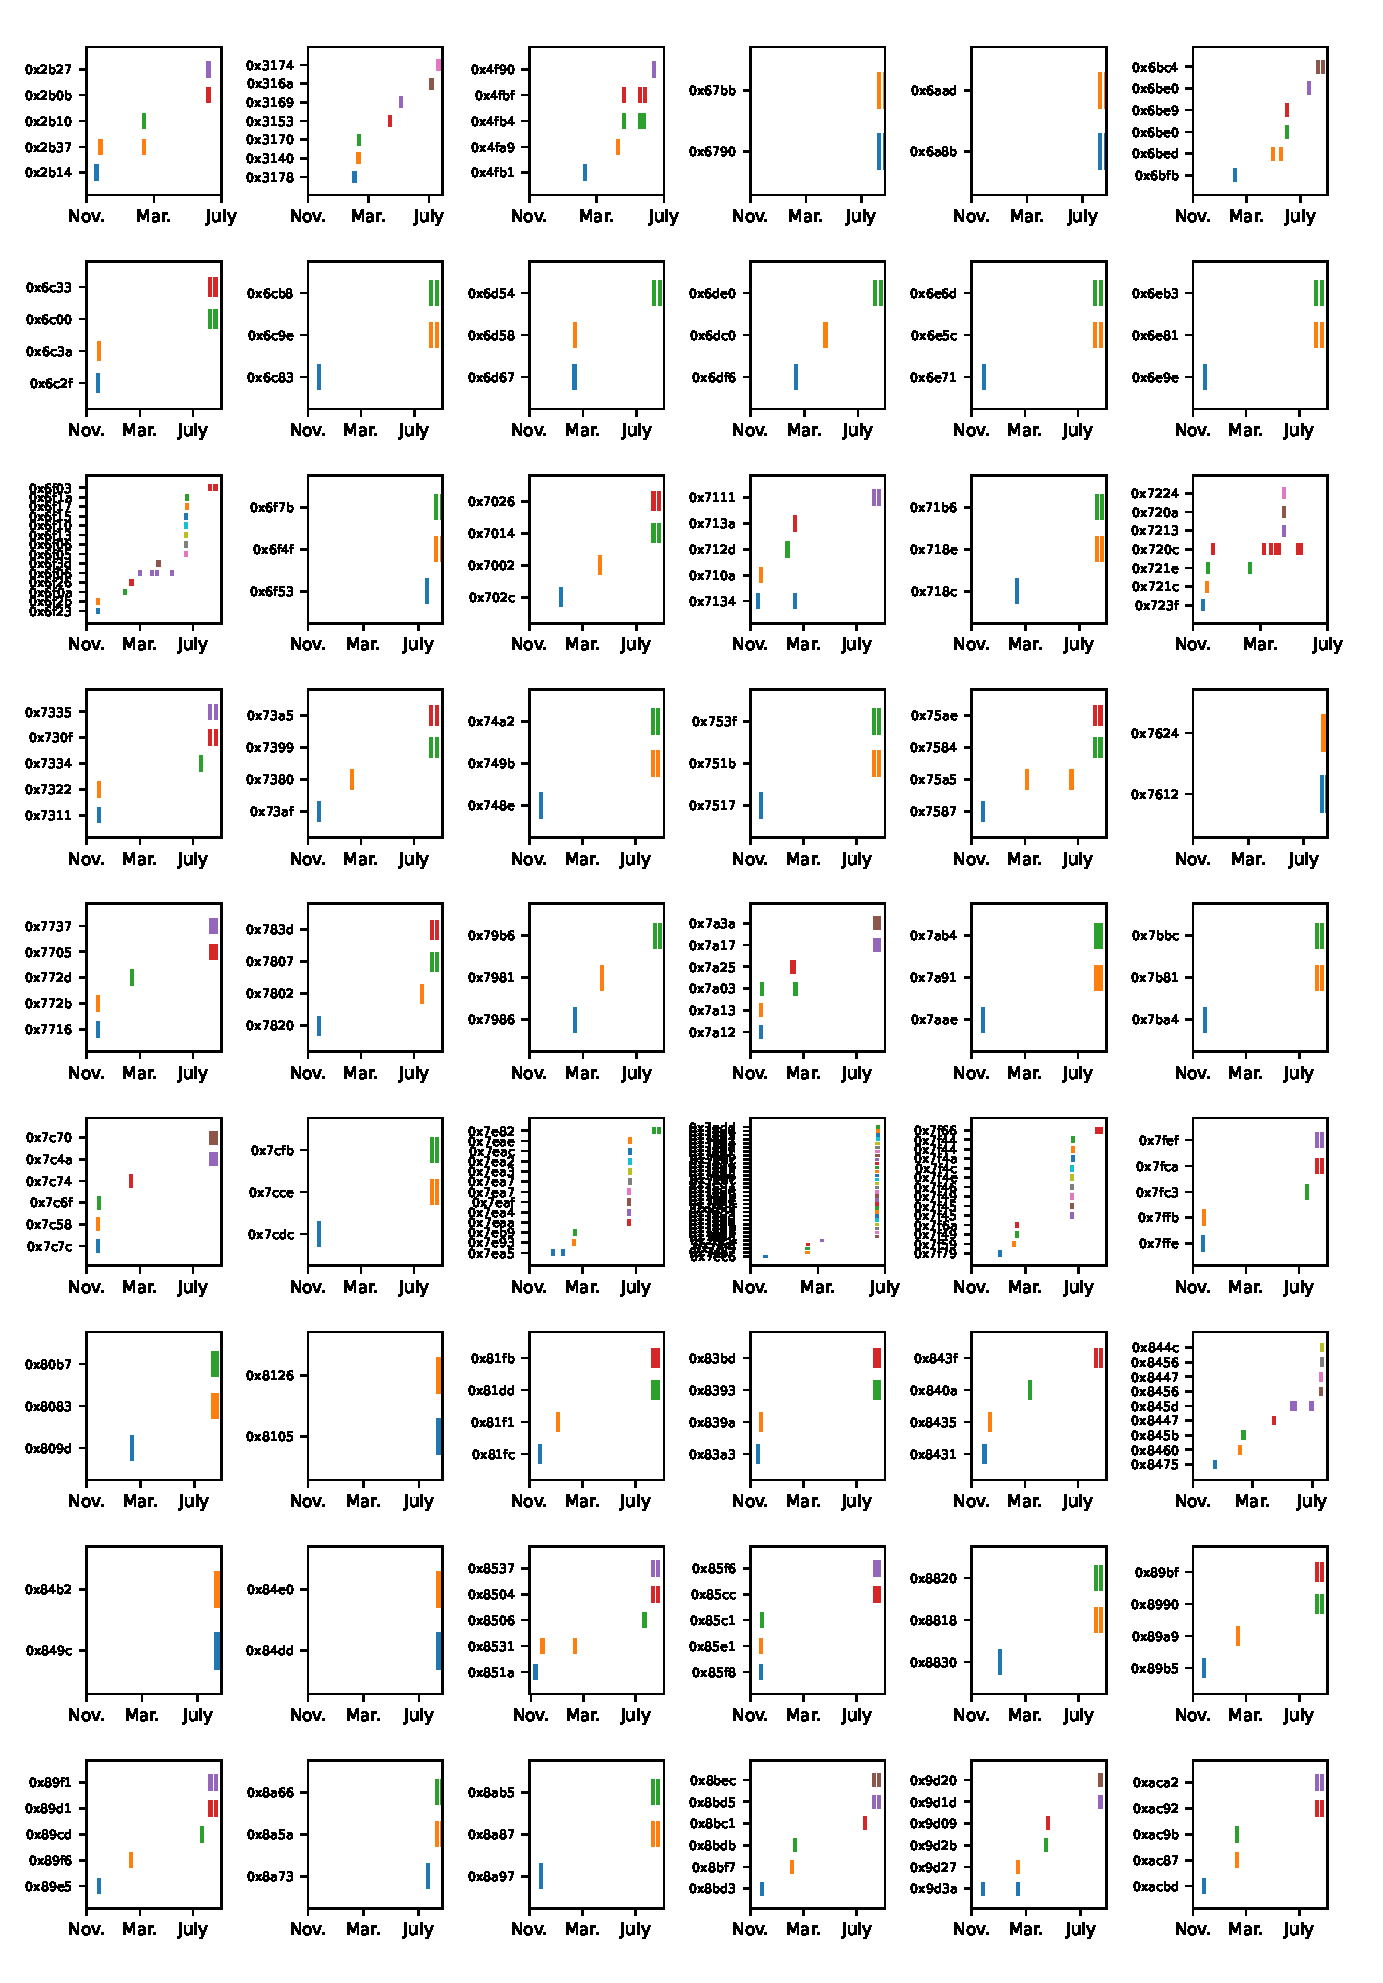
\includegraphics[width=\textwidth]{common/contested.eps}
    \caption{Stake update events in contested neighbourhoods}
    \label{event-plot}

  \end{center}
  \end{figure}
%
On many of the plots we can observe pairs of addresses that repeatedly top up at very similar times to one another.
%
We reproduce an example listing in Table \ref{event-listing}.
%
We posit that the most likely reason for this behaviour is that the same entity started numerous nodes at the same time and placed them in distinct 11-bit neighbourhoods.
%
Since we have sorted by 10-bit neighbourhoods we have caught multiple of these nodes in the same bin, making their activity look like contention.



\appendix
\section{Notation index}

% We ideally want something that's both a longtable (can span multiple pages) and tabularx
% (automatically breaks lines inside cells). This is probably provided by the LaTeX3
% package tabularray, which is not currently part of the build. Looking into it.

\renewcommand{\arraystretch}{1.3}
\begin{tabularx}{\textwidth}{lX}

  $\uR$ & Non-negative reals $[0,\infty)$. \\
  $\ssum_I$, $\ssum_{\hat{a}}$     & Sum over subset of entries of a vector with indices in $I$, resp.~over indices other than $a$. \\
  $\ssum^P$   & Sum masked by predicate $P$, i.e.~sum over indices $a$ such that $P(a)$. \\
  $\xi_{-a}$ & Restriction of a vector $\xi$ to the set of indices other than $a$. \\
  $\sim$ & As a superscript, indicates a random variable. \\
  $\Overlay\simeq\mathbb{F}_2^{256}$ & Node and data address space. \\
  $\Overlay(a,d)\subseteq\Overlay$ & Space of addresses sharing a $d$-bit prefix with $a\in\Overlay$. \\
  $\Xi$& Mechanism internal state space.   
  In the Swarm Protocol mechanism, $\Xi=\Xi^\Equity\times\Xi^\Active=(\uR\times\{0,1\})^\Overlay$. \\
  $\Xi^\Equity=\uR^\Overlay$ & Space of equity allocations. \\
  $\Xi^\Active = \{0,1\}^\Overlay$ & Space of active profiles, i.e.~subsets of nodes active in any given epoch. \\
  $\xi,\xi^\Equity,\xi^\Active$ & An element of $\Xi,\Xi^\Equity,\Xi^\Active$. \\
  $(\Omega,\Observable_\bullet,\Prob)$ & Filtered probability space of world histories. \\
  $\omega\in\Omega$ & A world history. \\
  $\Omega_0$ & Current world state, in case $\Omega\simeq \Omega_0^\N$ is a sequence space. \\
  $\omega^\mathrm{ex}$ & Exogenous components of world state. In our world, the principal components are $\omega^\mathrm{ex}=(R_\bullet,O_{\bullet,\bullet},\xi_{-a})$. \\
  $w(\xi)\in\Delta(\Overlay)$ & Allocation function. Several variants. \\
  $w^\Equity$   & Proportional allocation. \\
  $w^\tau$ & Proportional allocation masked by threshold $\tau>0$. \\
  $w^{\mathtt{SP}_\tau}$  & Swarm Protocol weighting: proportional weighting with threshold $\tau$ with liveness mask. \\
  $\Budget_{a,t}\in\uR$ & Budget of $a\in\Overlay$. \\
  $\tilde O_{a,t}$ & Operating cost of $a\in\Overlay$. \\
  $R_t$ & Redistributed revenue in $t$th epoch. \\
  $R_{a,t}$ & $a$'s share $w_a(\xi)R_t-O_{a,t}$ of redistributed revenue in $t$th epoch, after deducting costs. \\
  $\actions(\Budget)$ & Space of actions available with budget $\Budget$. \\
  $s\in\actions$ & An action/strategy. Has components $s_\mathtt{mint},s_\mathtt{div},s_\mathtt{on}$. \\
  $s_\mathtt{mint}\in\uR$ & Number of shares to mint under action $s$. \\
  $s_\mathtt{div}\in\uR$ & Balance to cash out under action $s$. \\
  $s_\Active\in\{0,1\}$   & Whether or not to be active under action $s$.

\end{tabularx}




\section{Ruin calculations}
\label{section:ruin-calculations}

We record here some calculations through which we attempted to obtain closed form ruin probabilities for the Swarm lottery payout system.
%
These calculations have not yielded useful results, and we expect the general approach to be superseded by more sophisticated methods such as those of \cite{asmussen2010ruin,albrecher2022blockchain}; nonetheless we include the working in case it proves useful at some point.

\begin{lemma}

  $\sum_{n=N}^\infty { n\choose k } x^n = {k+N \choose k} \frac{x^N}{(1-x)^{N+k+1}}$

\end{lemma}

Summing over all integer hitting times and starting capital, we find
\begin{align*}
  \sum_{k=1}^\infty\sum_{n\in\N} \Prob[T_0 = n\mid C_0=k]u^k &= \sum_{k\in\N}\sum_{n\in\N} \frac{k}{n} \Prob[C_n = 0\mid C_0=k]u^k 
\end{align*}
\begin{align*}
  &= \sum_{k\in\N}\sum_{n\in\N} \frac{k}{n} \Prob[k - n + R\tilde{U}_n = 0]u^k \\
  &= \sum_{\ell\in\N}\sum_{n=\ell R}^\infty \frac{n-\ell R}{n} \Prob[\tilde{U}_n = \ell]u^{n-\ell R}   \qquad (k=n-\ell R)\\
  &= \sum_{\ell\in\N} \left( \frac{p}{qu^R} \right)^\ell \sum_{n=\ell R}^\infty \left[ 
    {n\choose \ell} - R \frac{\ell}{n} {n\choose \ell} 
  \right](uq)^n \\
  &= \sum_{\ell\in\N} \left( \frac{p}{qu^R} \right)^\ell 
  \left( 
    \sum_{n=\ell R}^\infty {n\choose \ell} (uq)^n - 
    Ruq \sum_{n=\ell R - 1}^\infty {n\choose \ell-1} (uq)^n
  \right) \\
  &= \sum_{\ell\in\N} \left( 
    \frac{p}{qu^R} 
  \right)^\ell 
  \left(
    {\ell(R+1) \choose \ell} \frac{ (uq)^{\ell R} } {(1-uq)^{\ell(R+1)+1} } - 
    Ruq {\ell(R+1)-2 \choose \ell - 1} \frac { (uq)^{\ell R-1} } { (1-uq)^{\ell(R+1) -1} }
  \right) \\
  &= \sum_{\ell\in\N} \left( 
    \frac{p(uq)^R}{qu^R(1-uq)^{R+1}} 
  \right)^\ell 
  \left(
    {\ell(R+1) \choose \ell} (1-uq)^{-1} - 
    R {\ell(R+1)-2 \choose \ell - 1} (1-uq)
  \right)  \\
  &= \sum_{\ell\in\N} \left( 
    \frac{pq^{R-1}}{(1-uq)^{R+1}} 
  \right)^\ell 
  \left(
    {\ell(R+1) \choose \ell} (1-uq)^{-1} - 
    R {\ell(R+1)-2 \choose \ell - 1} (1-uq)
  \right)
\end{align*}

We don't know a closed form for the series $\sum_\ell { k\ell \choose \ell }x^\ell $ for general $k>2$.
%
However, for $k=2$ the coefficients are the central binomial coefficients, which we can study in closed form (although this case $R=1$ is not very important in practice).
%
\begin{align*}
  &= \sum_{\ell\in\N} \left( 
    \frac{p}{(1-uq)^{2}} 
  \right)^\ell 
  \left(
    {2\ell \choose \ell} (1-uq)^{-1} - 
    R {2(\ell-1) \choose \ell - 1} (1-uq)
  \right) \\
  &= \sum_{\ell\in\N} \left( 
    \frac{p}{(1-uq)^{2}} 
  \right)^\ell 
  \left(
    {2\ell \choose \ell} \frac{1-Rp}{1-uq}
  \right) \\
  &= \frac{1-Rp}{1-uq}\left(
    1 - 4\cdot \frac{p}{(1-uq)^{2}}
  \right)^{-\frac{1}{2}} 
\end{align*}

To solve for the eventual ruin probability, we need to specialise to fixed $k>0$ and sum over $n\in\N$.
%
In principle, we can extract this from the generating function by applying $\frac{\partial^k}{k!\partial u^k}$ and evaluating at $u=0$.
%
However, without any clear sign this is going to produce anything userful, we put aside the effort.

%\begin{align*}
%  \sum_{k\in\N}\sum_{n\in\N} \Prob[T_0 = n\mid C_0=k]u^k &= \left( 1- \frac{pu^{-R}}{(1-p)(1-u(1-p))} \right)^{-1}((1-u(1-p))^{-1}-R) 
%\end{align*}
%Then applying the $k$th derivative, we get


%?
%\[
%  \Prob(T_0 <\infty\mid C_0=k) = (1-p)^{-k}(p^{-1}-R)
%\]